\documentclass[12pt, a4paper]{article}
\usepackage[utf8]{inputenc}

\usepackage[a4paper,top=3cm,bottom=2cm,left=2.5cm,right=2.5cm,marginparwidth=1.75cm]{geometry}
%\usepackage[utf8]{inputenc}
%\usepackage[T1]{fontenc}
\usepackage{adjustbox}
\usepackage{amsmath}
\usepackage{amssymb}
\usepackage[ngerman, english]{babel}
\usepackage{booktabs}
\usepackage{csquotes}
\usepackage{float}
\usepackage{graphicx}
\usepackage{longtable}
\usepackage{lscape}
\usepackage{subfig,caption}
\usepackage{tabularx}
\usepackage{threeparttablex}
\usepackage{xcolor}
\usepackage{xtab}
\usepackage{hyperref}

% everything concerning biblatex

\usepackage[backend = biber,
            style=authoryear-icomp,
            citestyle=authoryear-comp,
            url=false,
            isbn=false,
            doi=false,
            maxcitenames=2,
            uniquelist=false,
            date=year,
            uniquename=false]{biblatex}

\addbibresource{References.bib} % TBD

% Setup
\graphicspath{{../1_Figures/}}

% new environment

\newenvironment{subcaption}
{\strut
\vspace{-5pt}
\begin{minipage}[b]{0.9\textwidth}
  \hspace*{-\parindent}
  \footnotesize}
 {\end{minipage}}

 % Title

\title{Global inequality in carbon-intensive consumption}
\author{Leonard Missbach\thanks{Mercator Research Institute on Global Commons and Climate Change, Berlin, Germany; Department Economics of Climate Chagne, Technische Universität Berlin, Berlin, Germany}}
\date{January 2023}

\begin{document}

\maketitle
\begin{abstract}
  In this study ...
\end{abstract}

\smallskip

\noindent \small \textit{Keywords:} Climate mitigation, inequality, poverty

\noindent \small \textit{JEL Codes:}

\thispagestyle{empty}
\clearpage
\setcounter{page}{1}

\section{Main} \label{sec:main}

\clearpage

\section{Data and Methods} \label{sec:data_and_methods}

\clearpage

\printbibliography

\clearpage

\appendix

\section{Appendix} \label{sec:appendix}

\renewcommand\thefigure{\thesection.\arabic{figure}}
\renewcommand\thetable{\thesection.\arabic{table}}
\setcounter{figure}{0}
\setcounter{table}{0}

\subsection{Supplementary figures} \label{sec:figures}

\begin{figure}[ht!]
  \centering
  \caption{Engel curves: expenditure shares over total household expenditures - Part A} \label{fig:A1}
  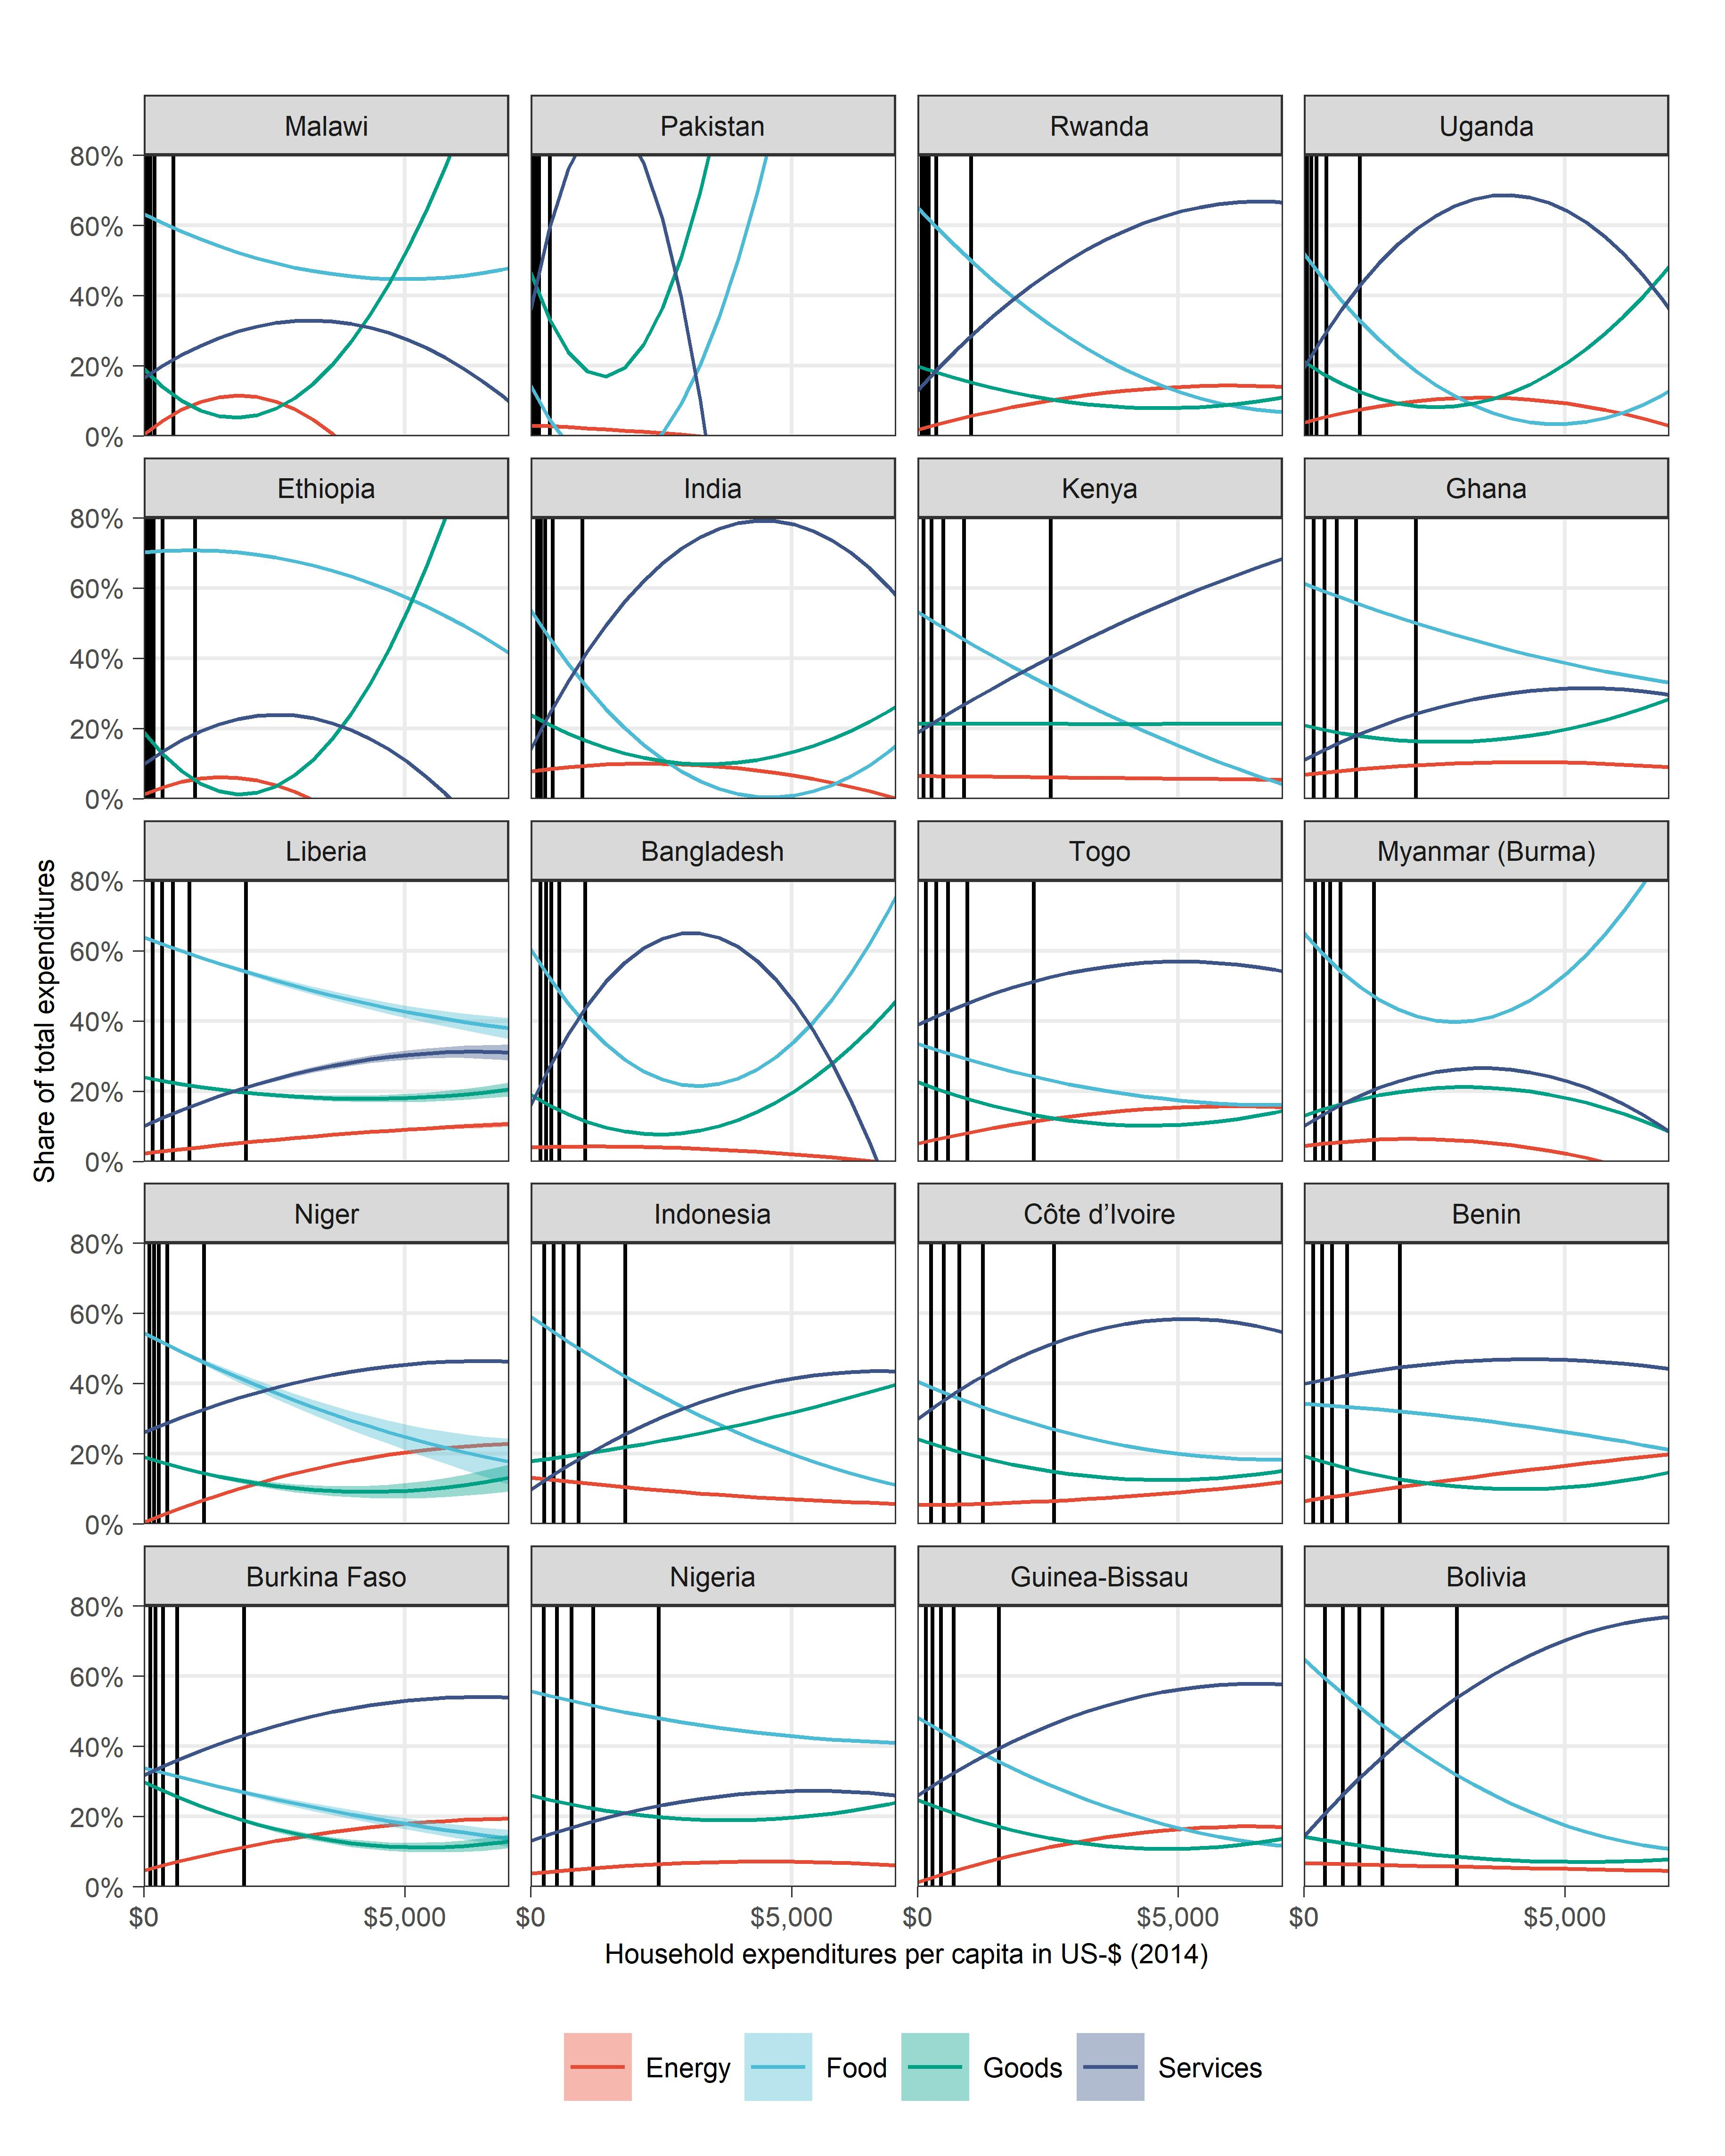
\includegraphics{Analysis_Parametric_Engel_Curves/Parametric_EC_0_A}
  \begin{subcaption}
    This figure displays ...
  \end{subcaption}

\end{figure}

\clearpage

\begin{figure}[ht!]
  \centering
  \caption{Engel curves: expenditure shares over total household expenditures - Part B} \label{fig:A2}
  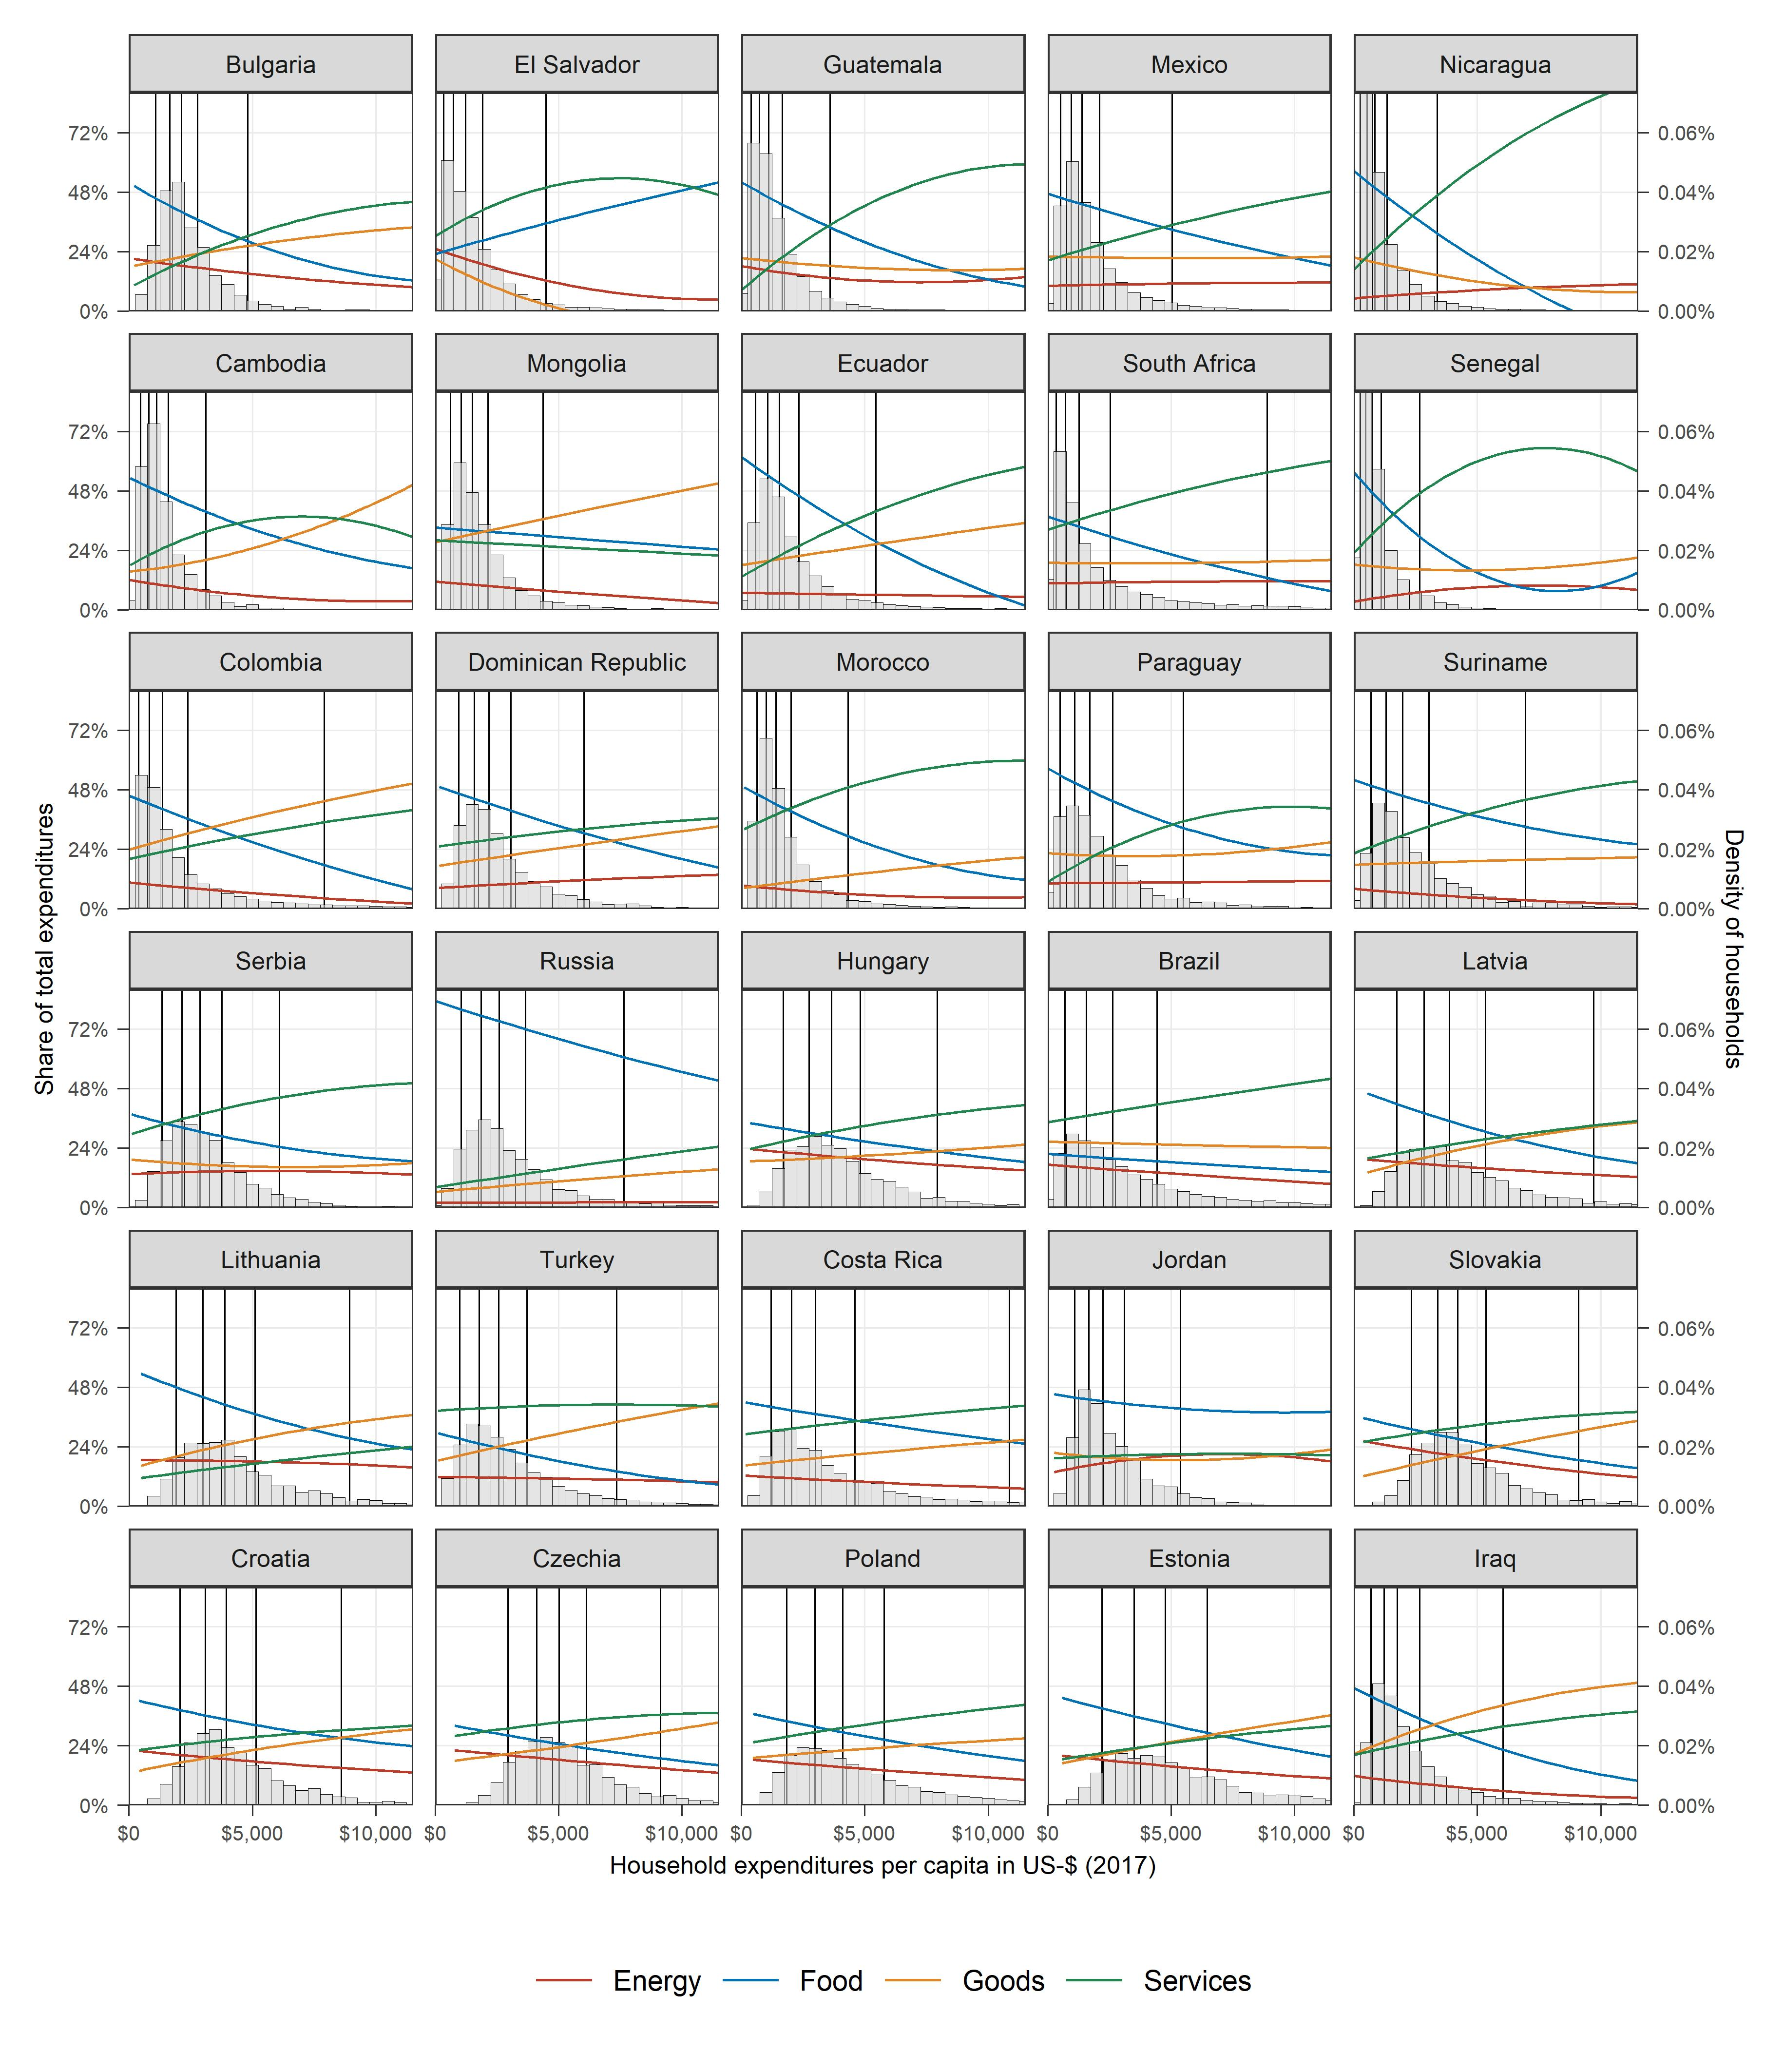
\includegraphics{Analysis_Parametric_Engel_Curves/Parametric_EC_0_B}
  \begin{subcaption}
    This figure displays ...
  \end{subcaption}

\end{figure}

\clearpage

\begin{figure}[ht!]
  \centering
  \caption{Engel curves: expenditure shares over total household expenditures - Part C} \label{fig:A3}
  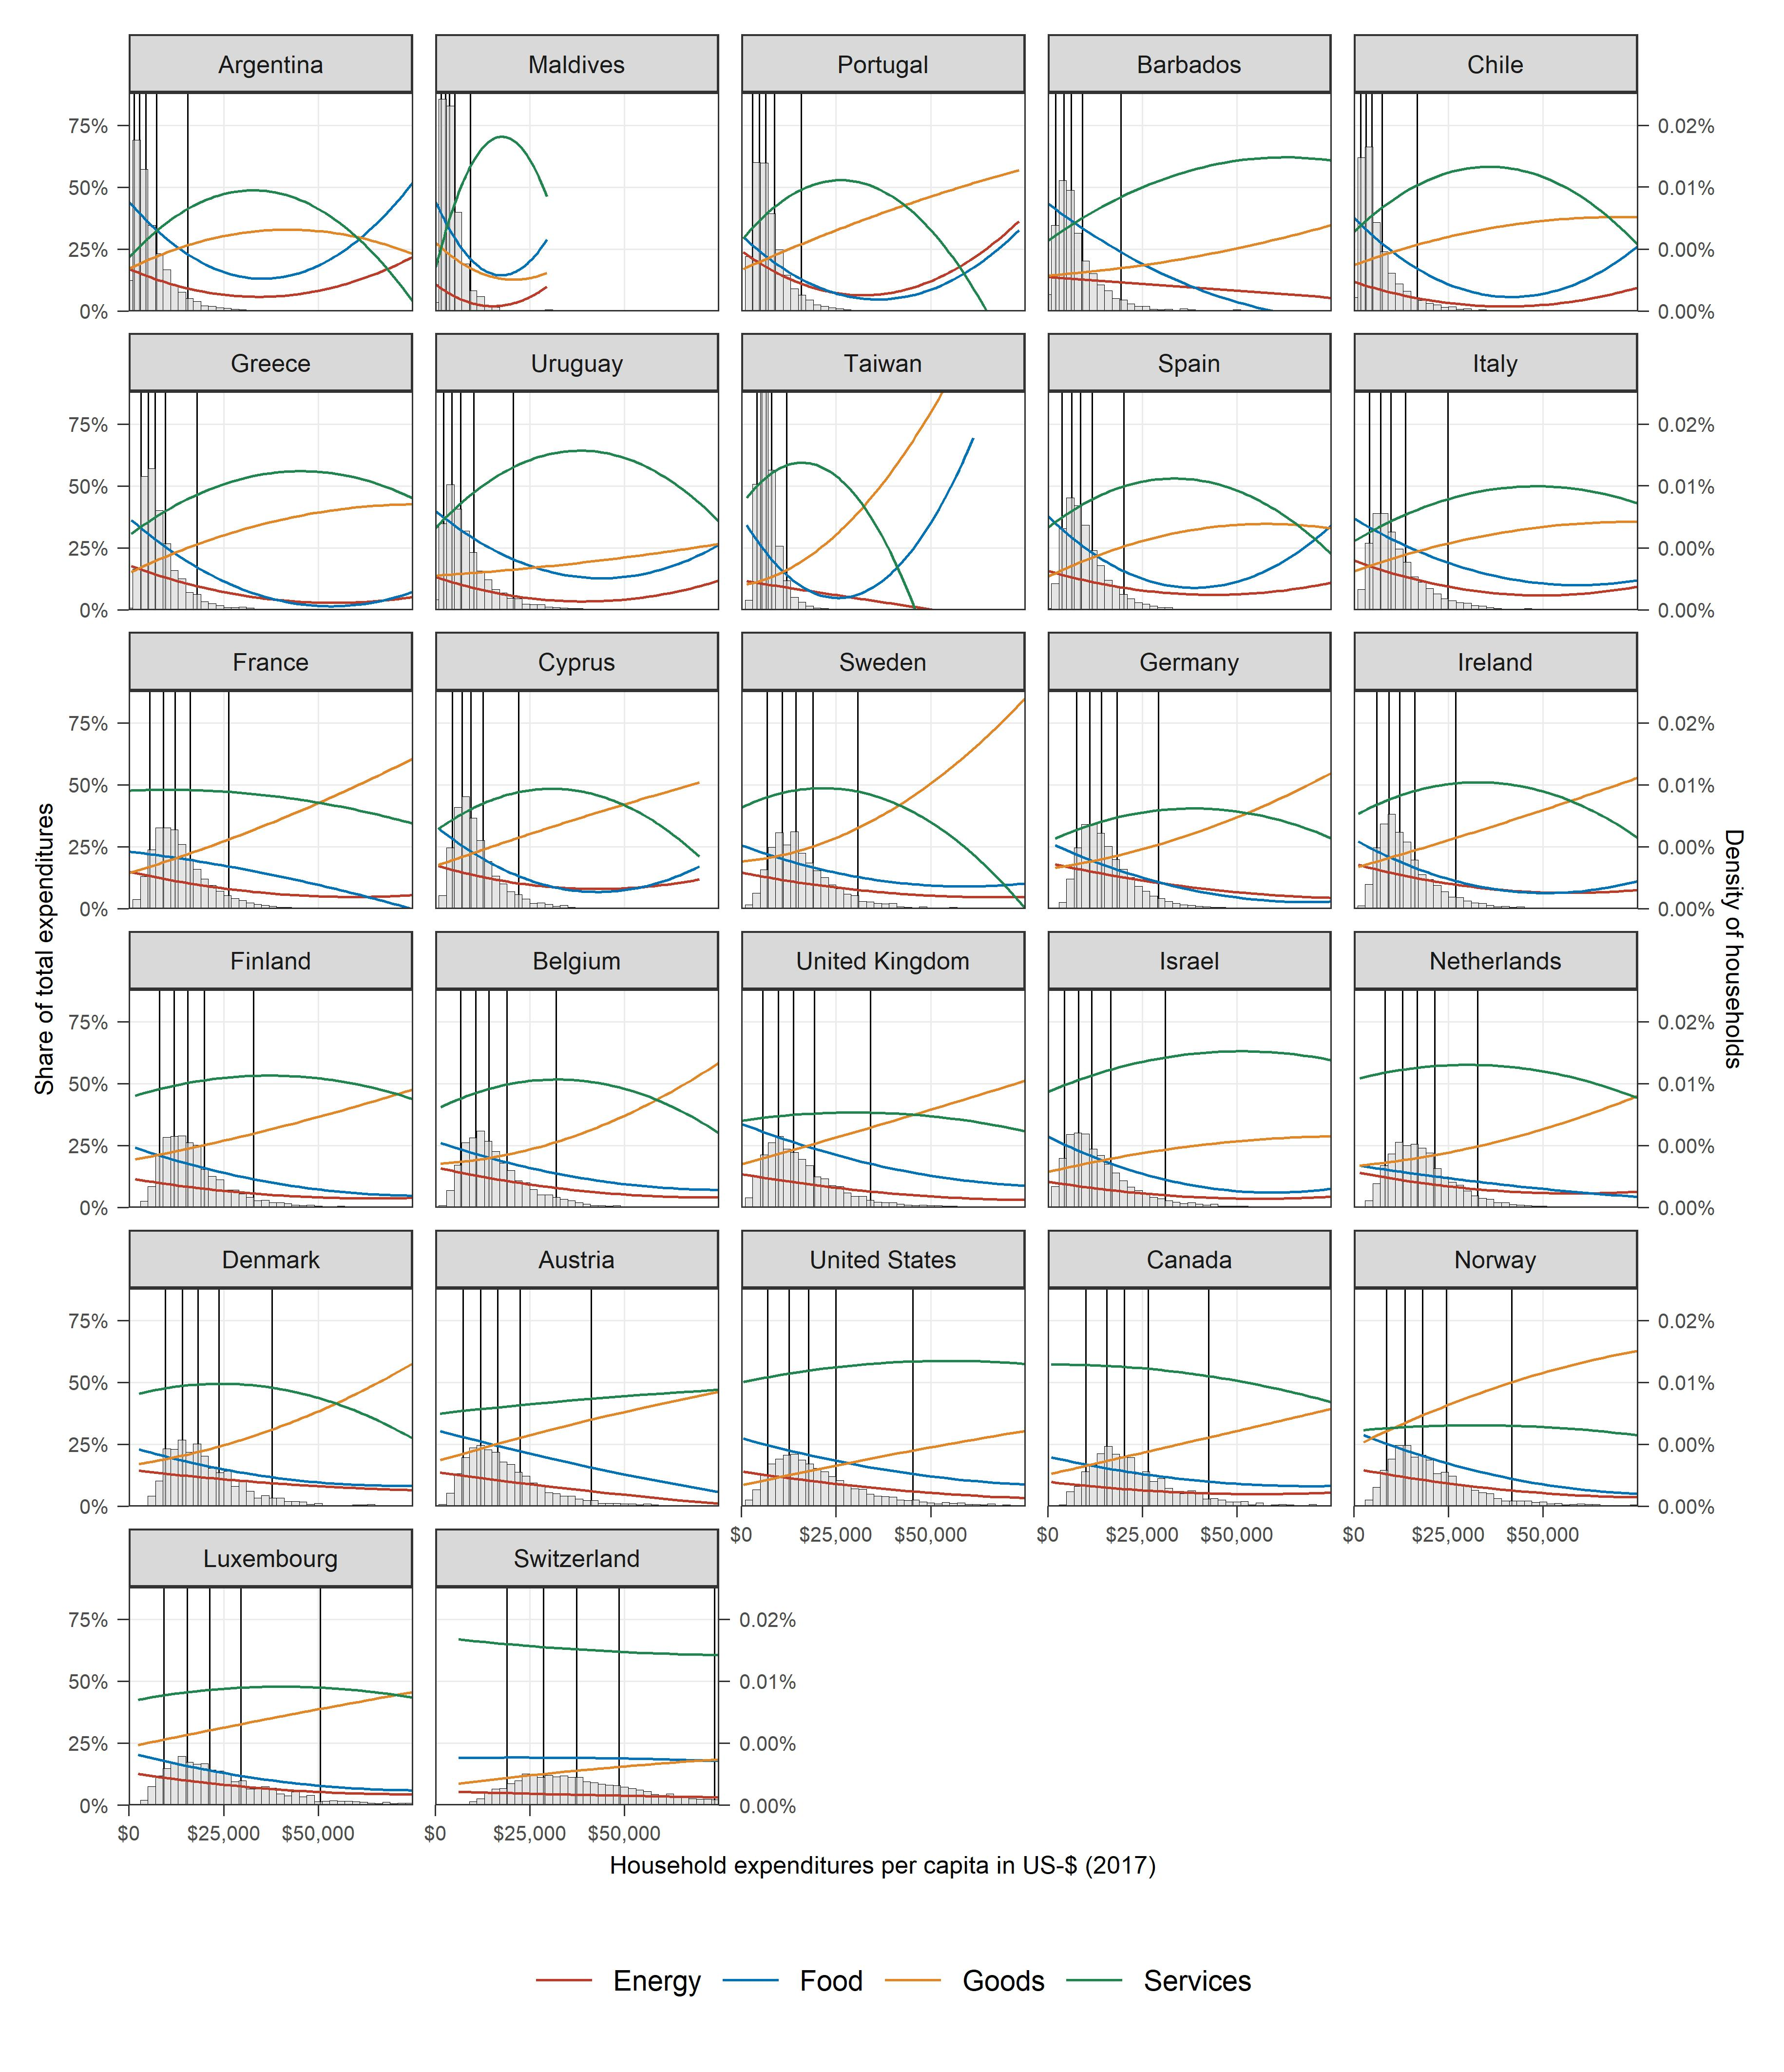
\includegraphics{Analysis_Parametric_Engel_Curves/Parametric_EC_0_C}
  \begin{subcaption}
    This figure displays ...
  \end{subcaption}

\end{figure}

\clearpage

\begin{figure}[ht!]
  \centering
  \caption{Engel curves: expenditure shares over total household expenditures - Part D} \label{fig:A4}
  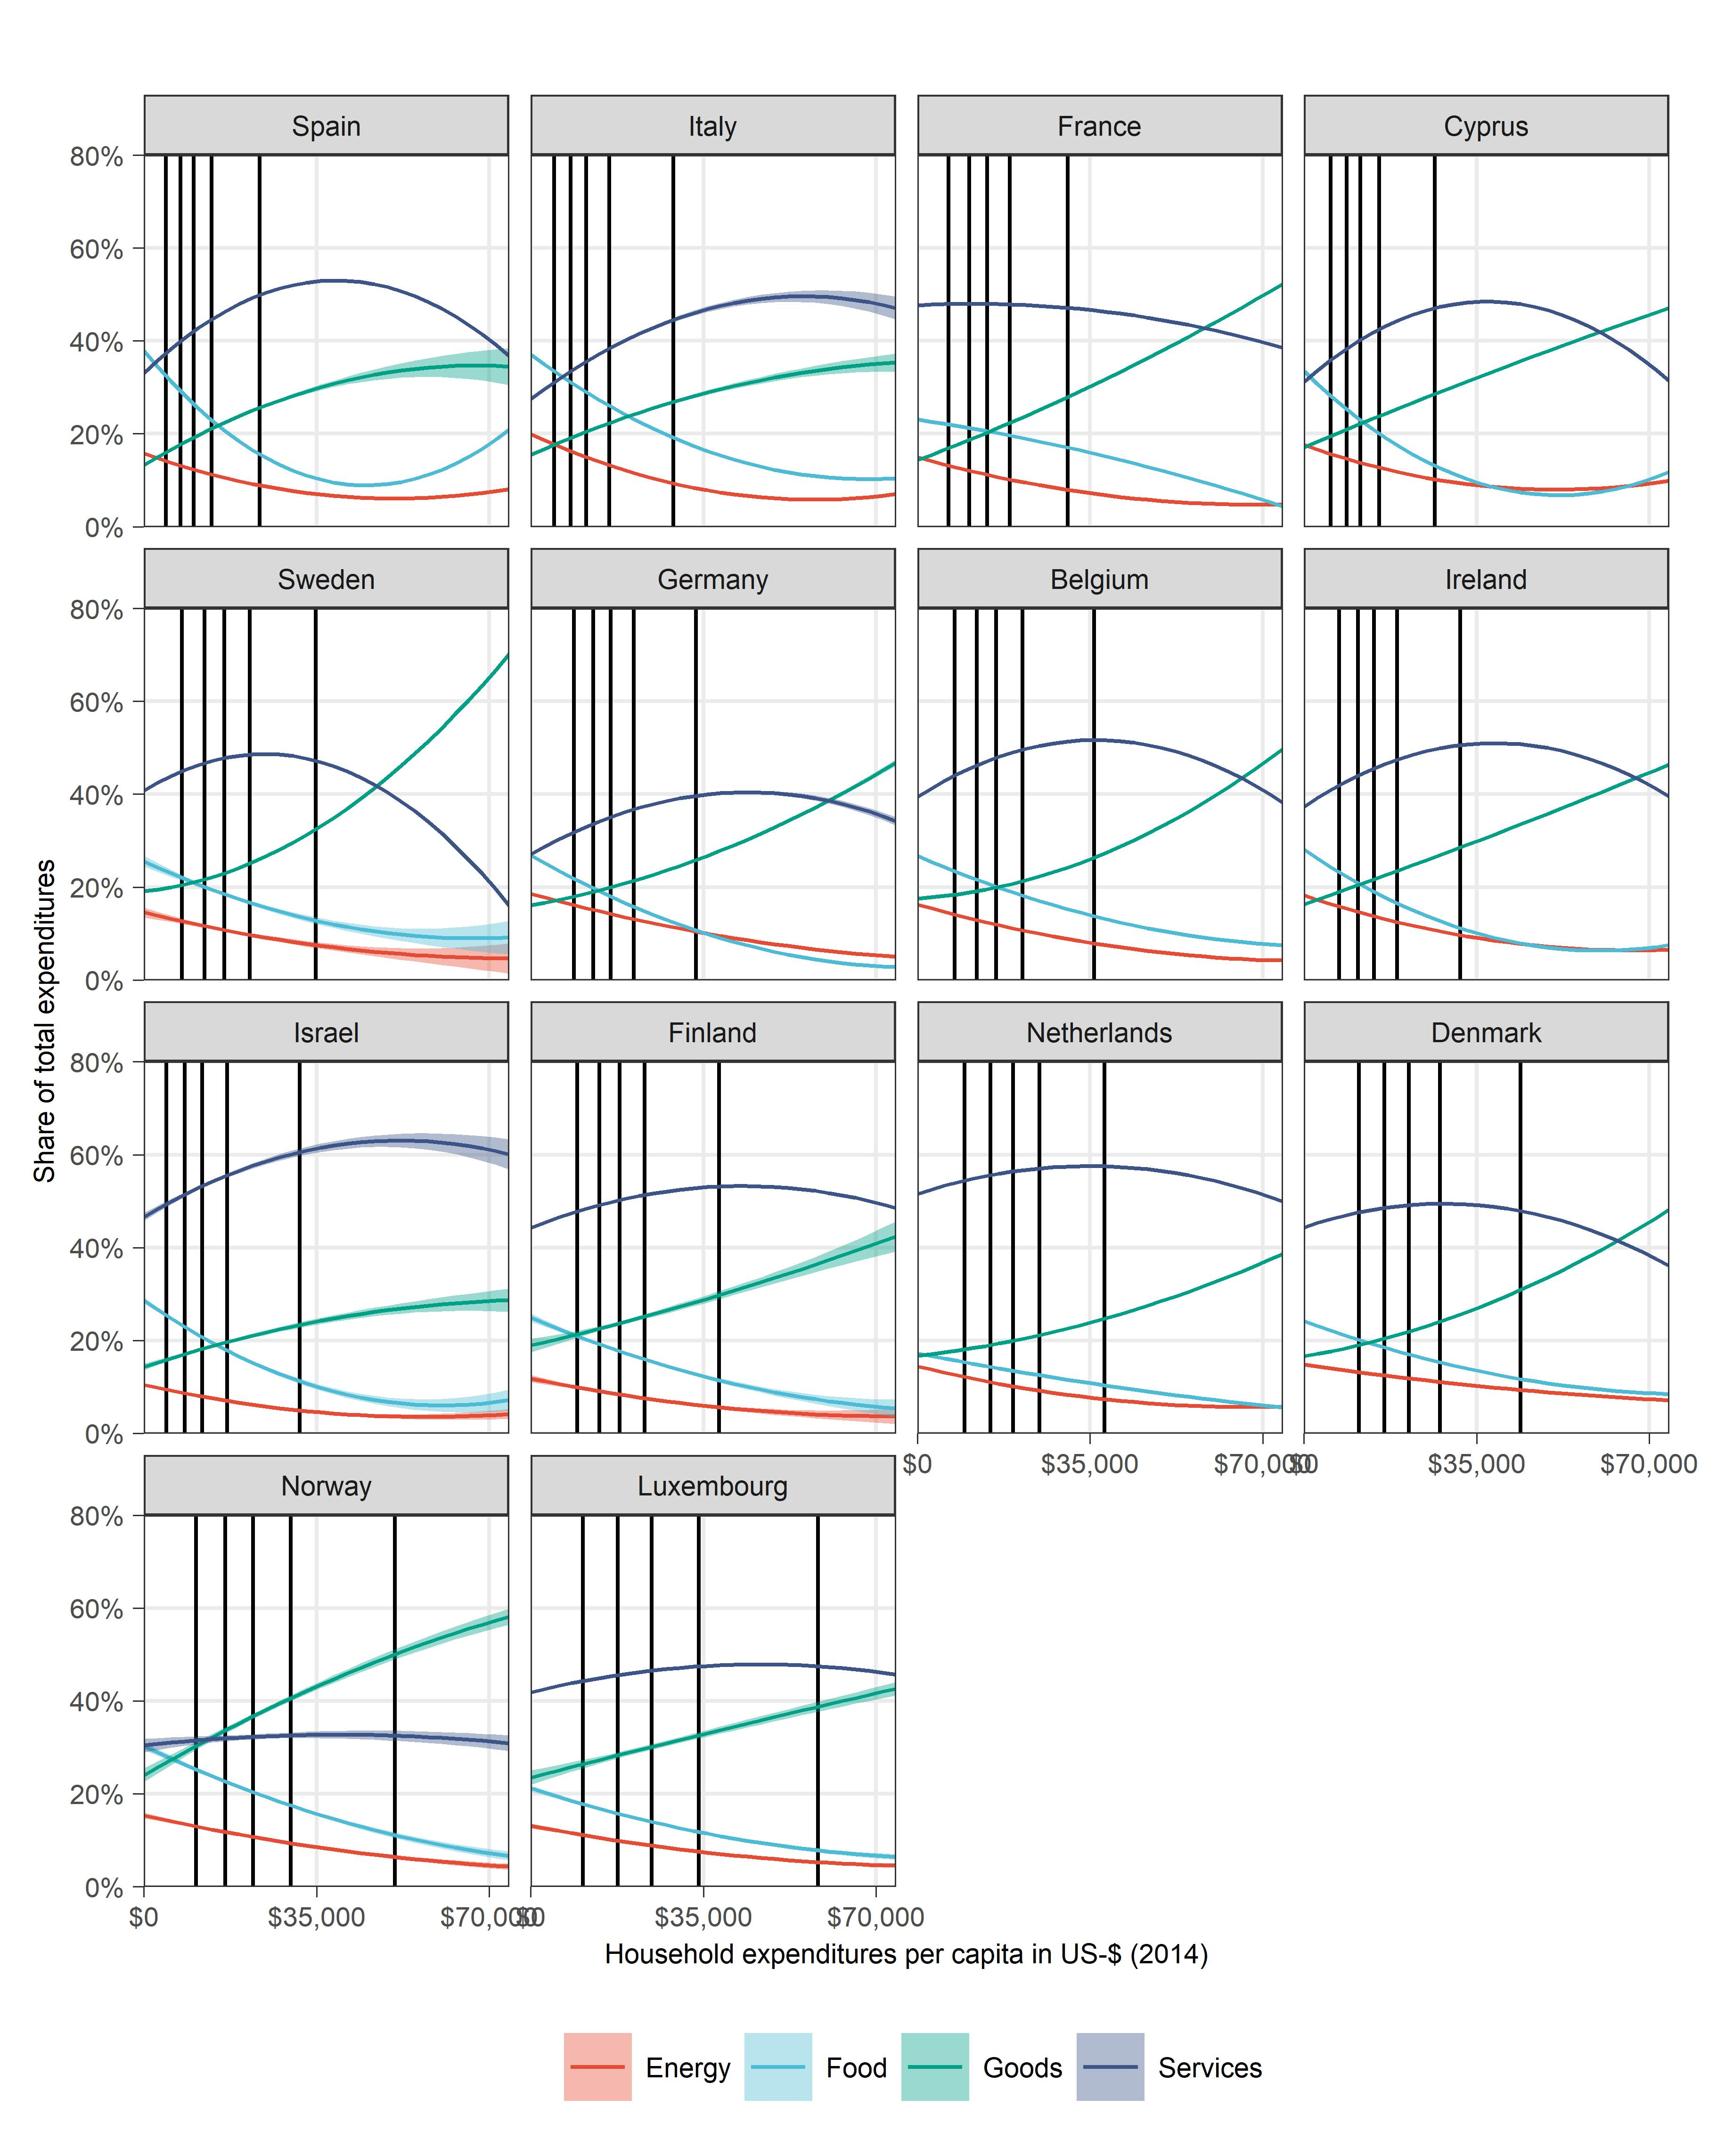
\includegraphics{Analysis_Parametric_Engel_Curves/Parametric_EC_0_D}
  \begin{subcaption}
    This figure displays ...
  \end{subcaption}

\end{figure}

\clearpage

\begin{figure}[ht!]
  \centering
  \caption{Carbon intensity of consumption over total household expenditures - Part A} \label{fig:B1}
  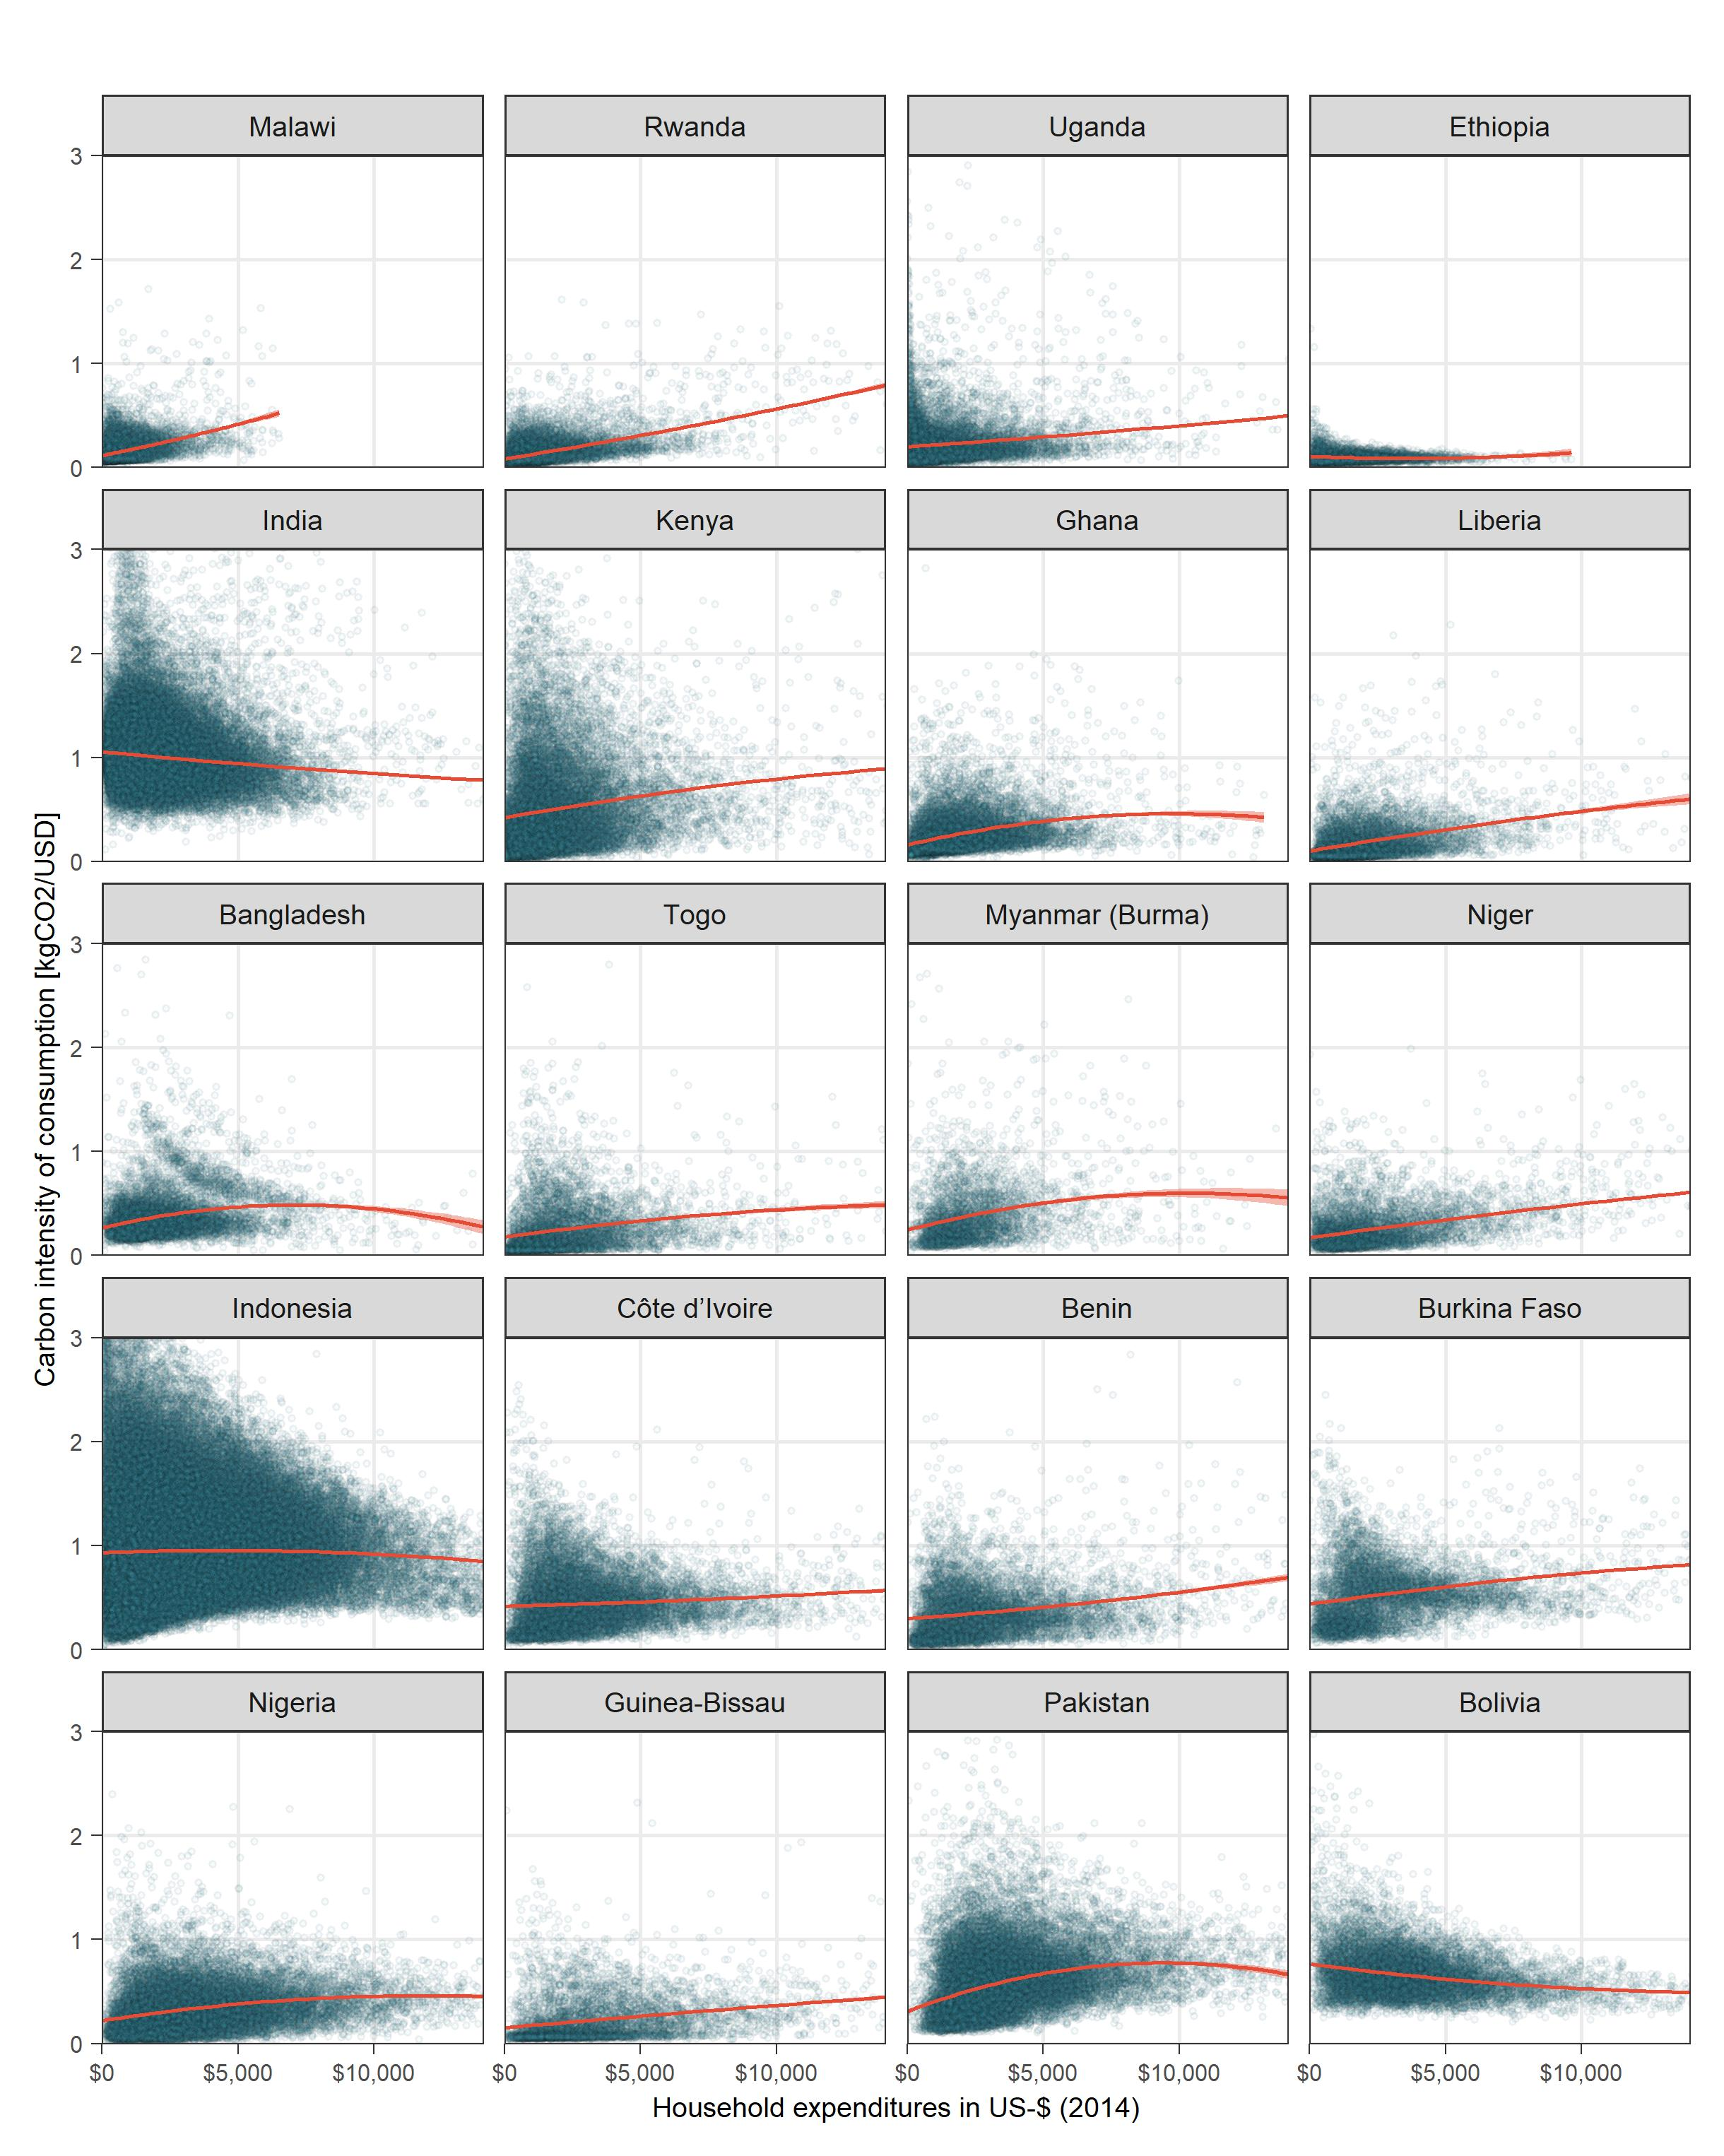
\includegraphics{Analysis_Carbon_Intensity_Curve/All_Panel_A}
  \begin{subcaption}
    This figure displays ...
  \end{subcaption}

\end{figure}

\clearpage

\begin{figure}[ht!]
  \centering
  \caption{Carbon intensity of consumption over total household expenditures - Part B} \label{fig:B2}
  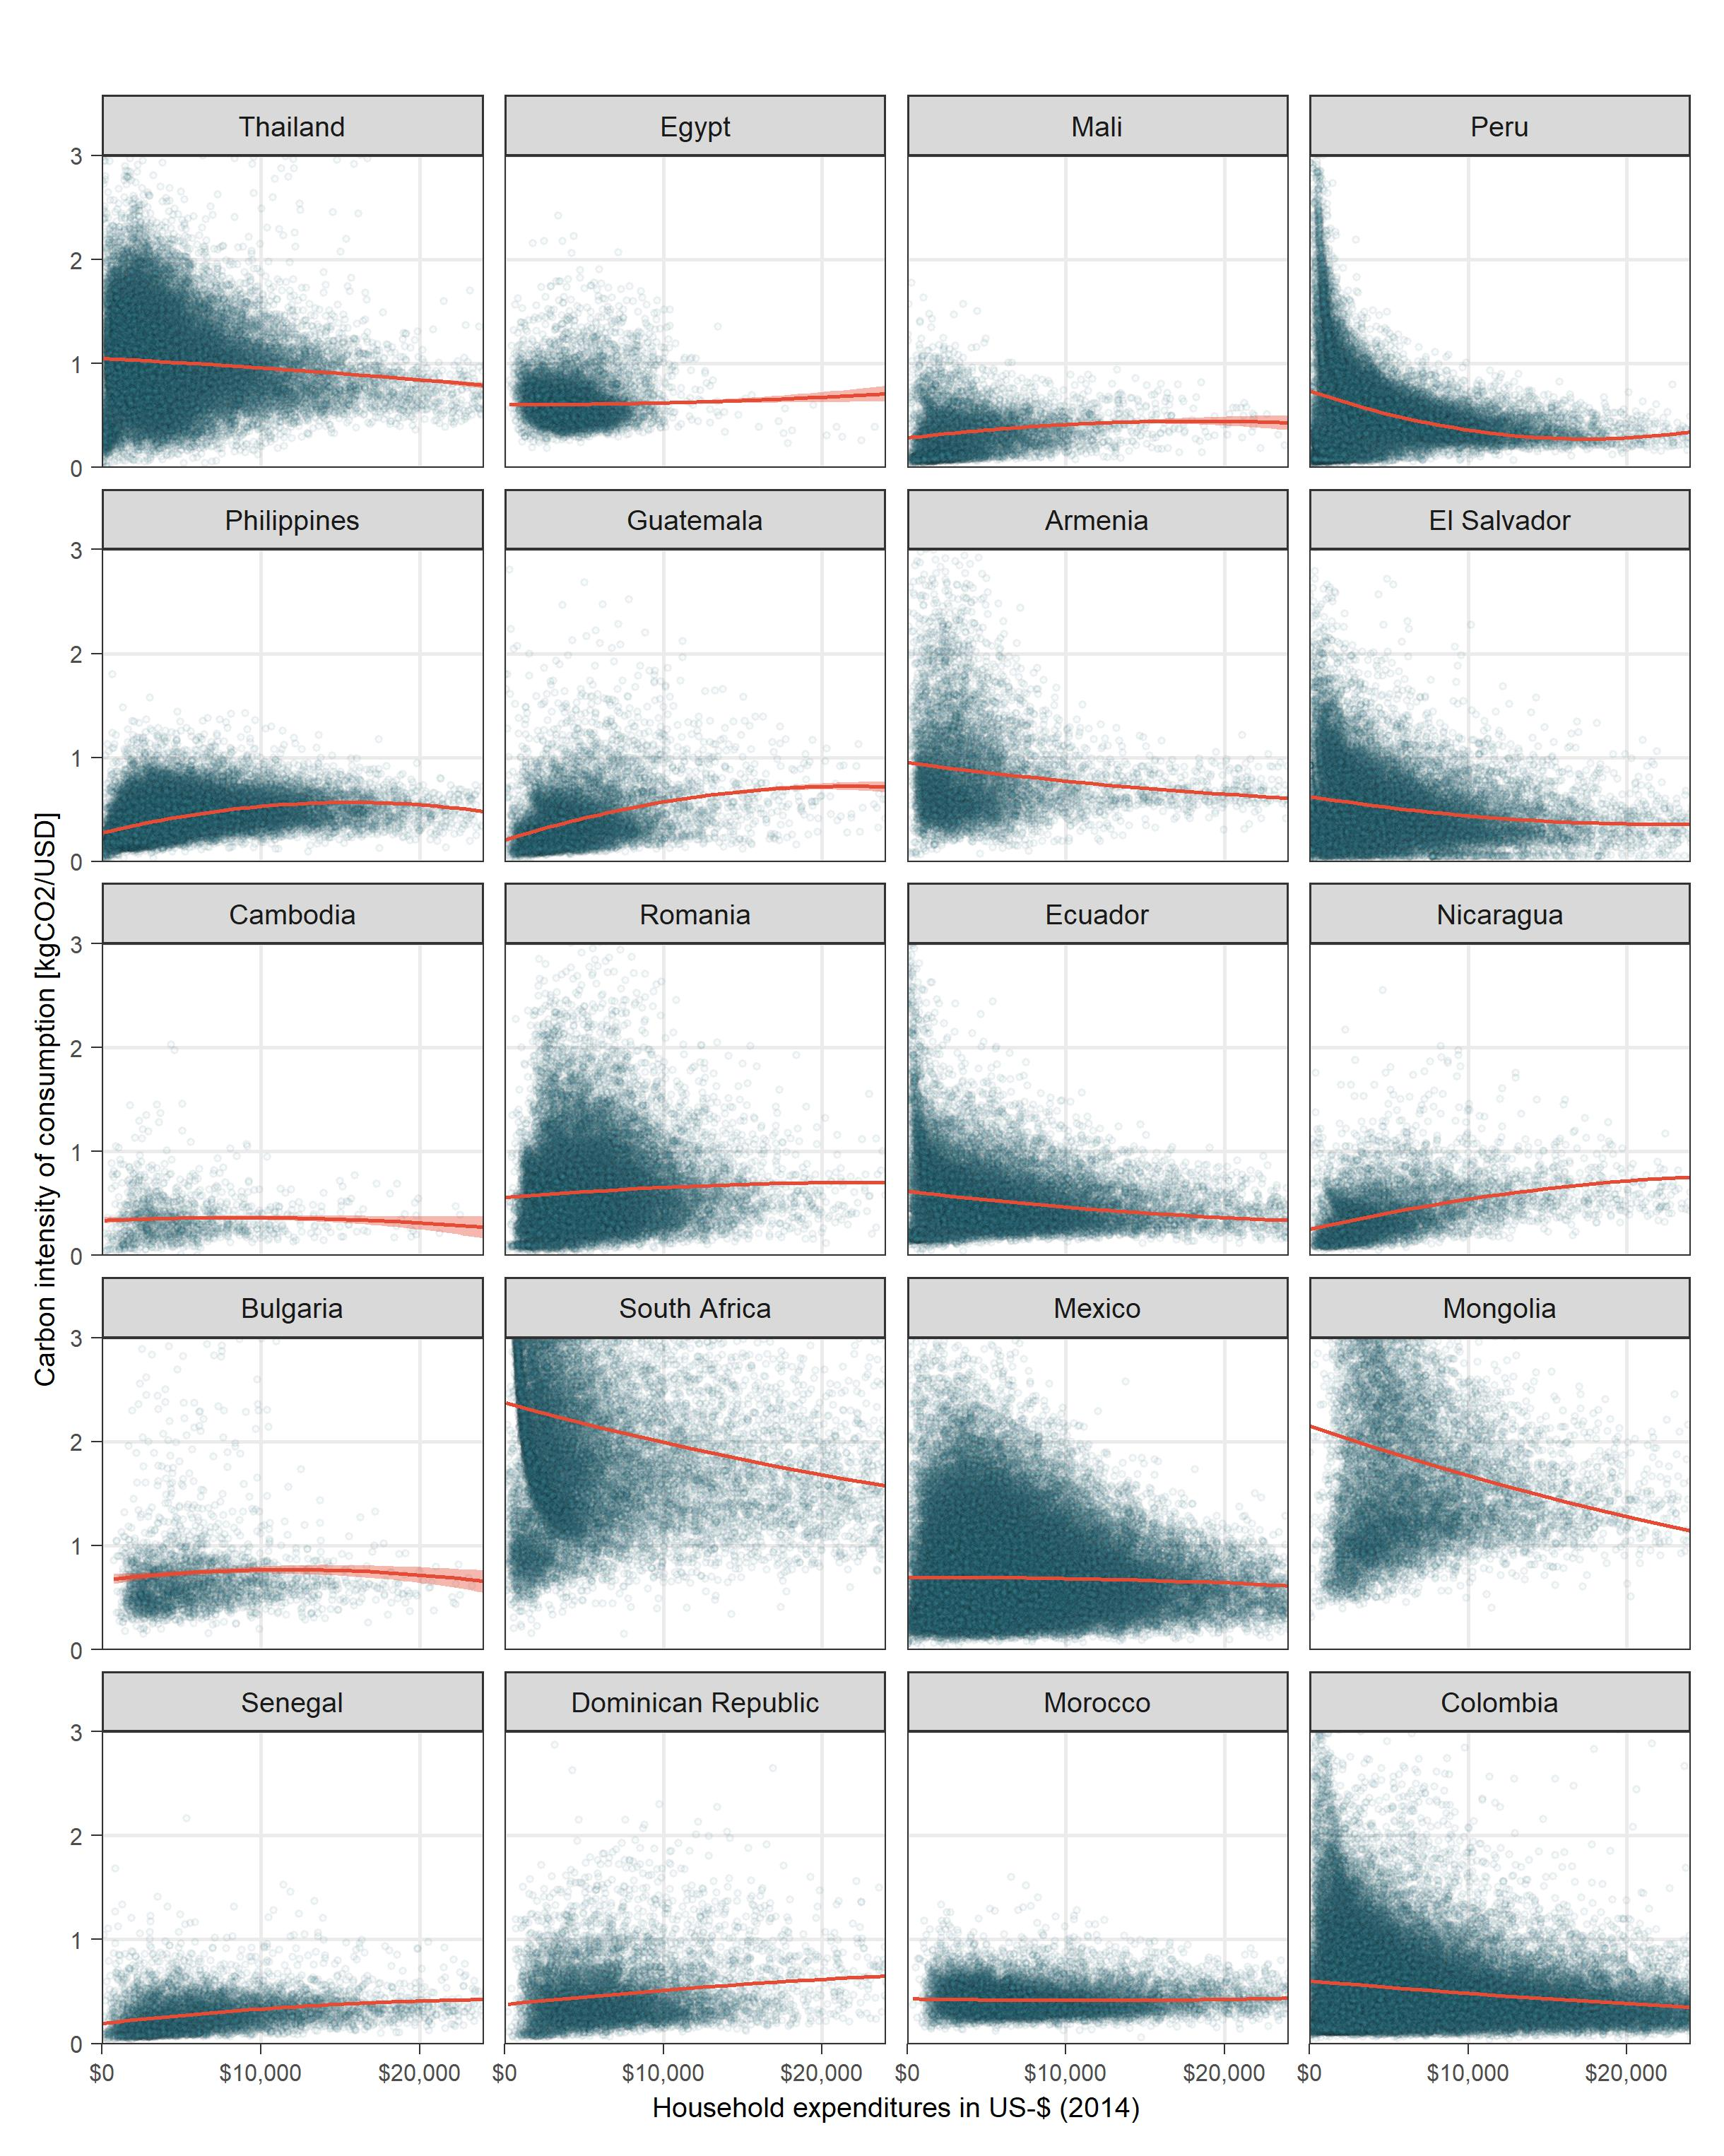
\includegraphics{Analysis_Carbon_Intensity_Curve/All_Panel_B}
  \begin{subcaption}
    This figure displays ...
  \end{subcaption}

\end{figure}

\clearpage

\begin{figure}[ht!]
  \centering
  \caption{Carbon intensity of consumption over total household expenditures - Part C} \label{fig:B3}
  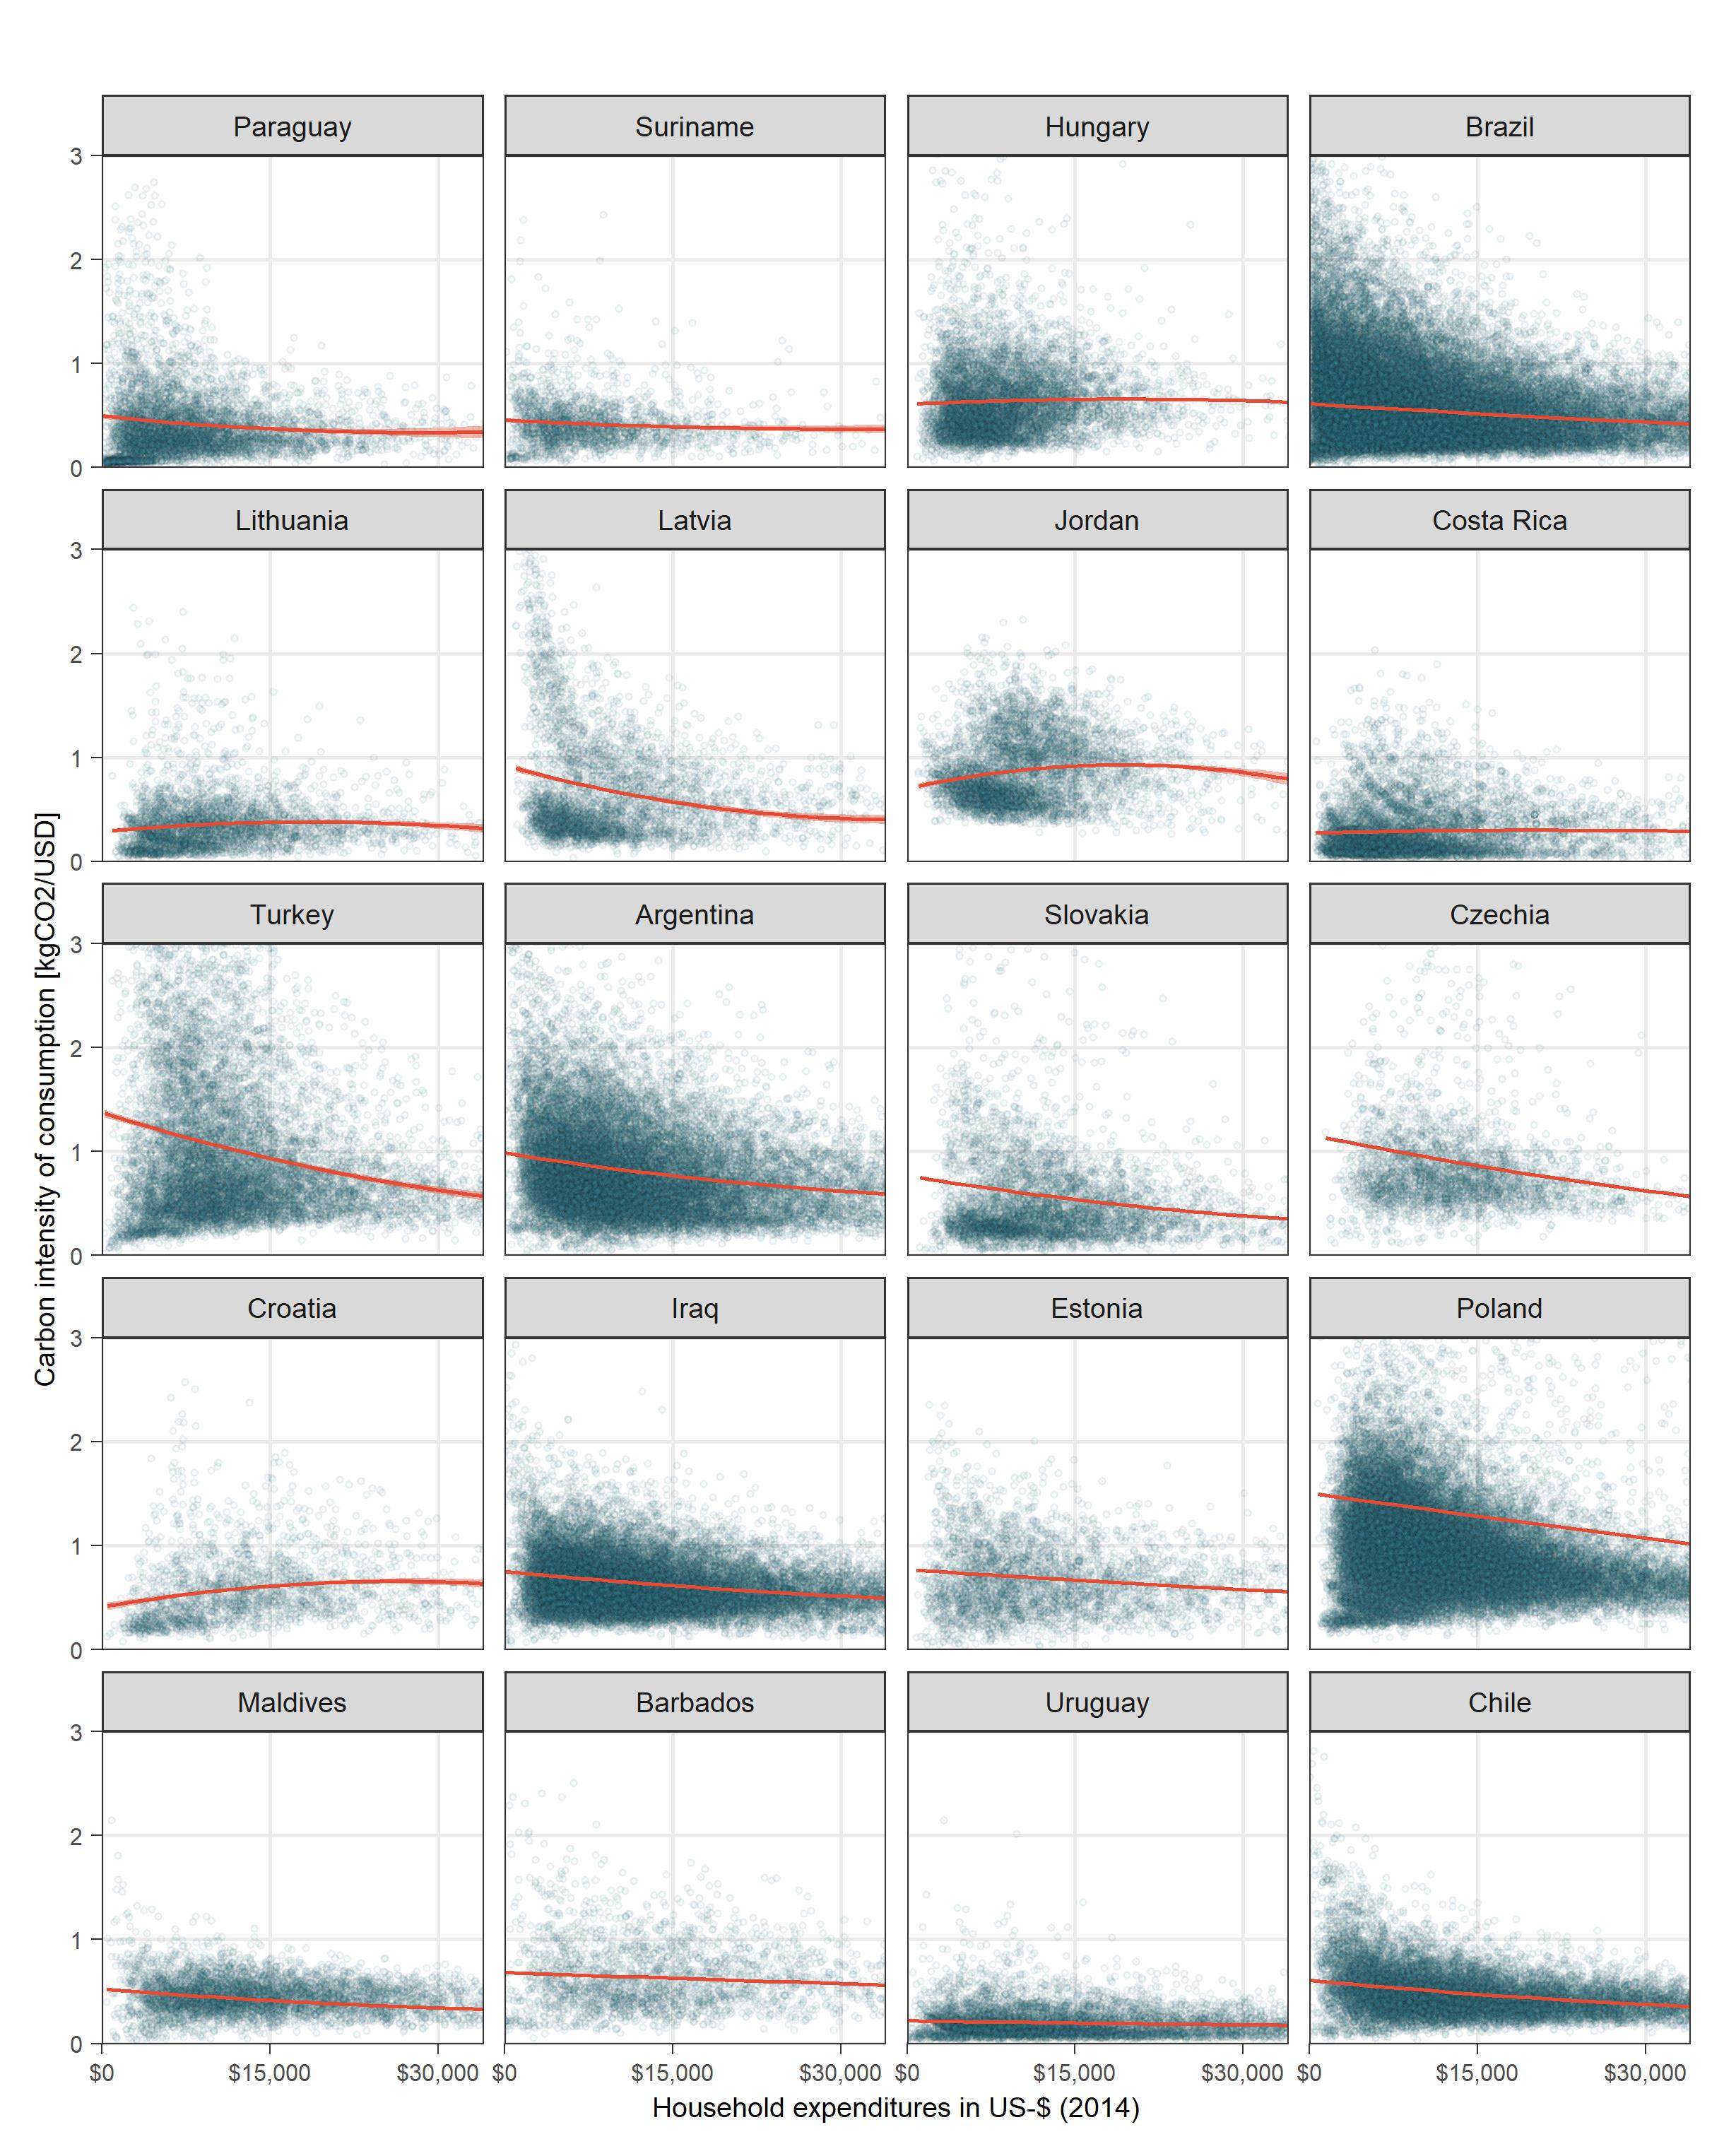
\includegraphics{Analysis_Carbon_Intensity_Curve/All_Panel_C}
  \begin{subcaption}
    This figure displays ...
  \end{subcaption}

\end{figure}

\clearpage

\begin{figure}[ht!]
  \centering
  \caption{Carbon intensity of consumption over total household expenditures - Part D} \label{fig:B4}
  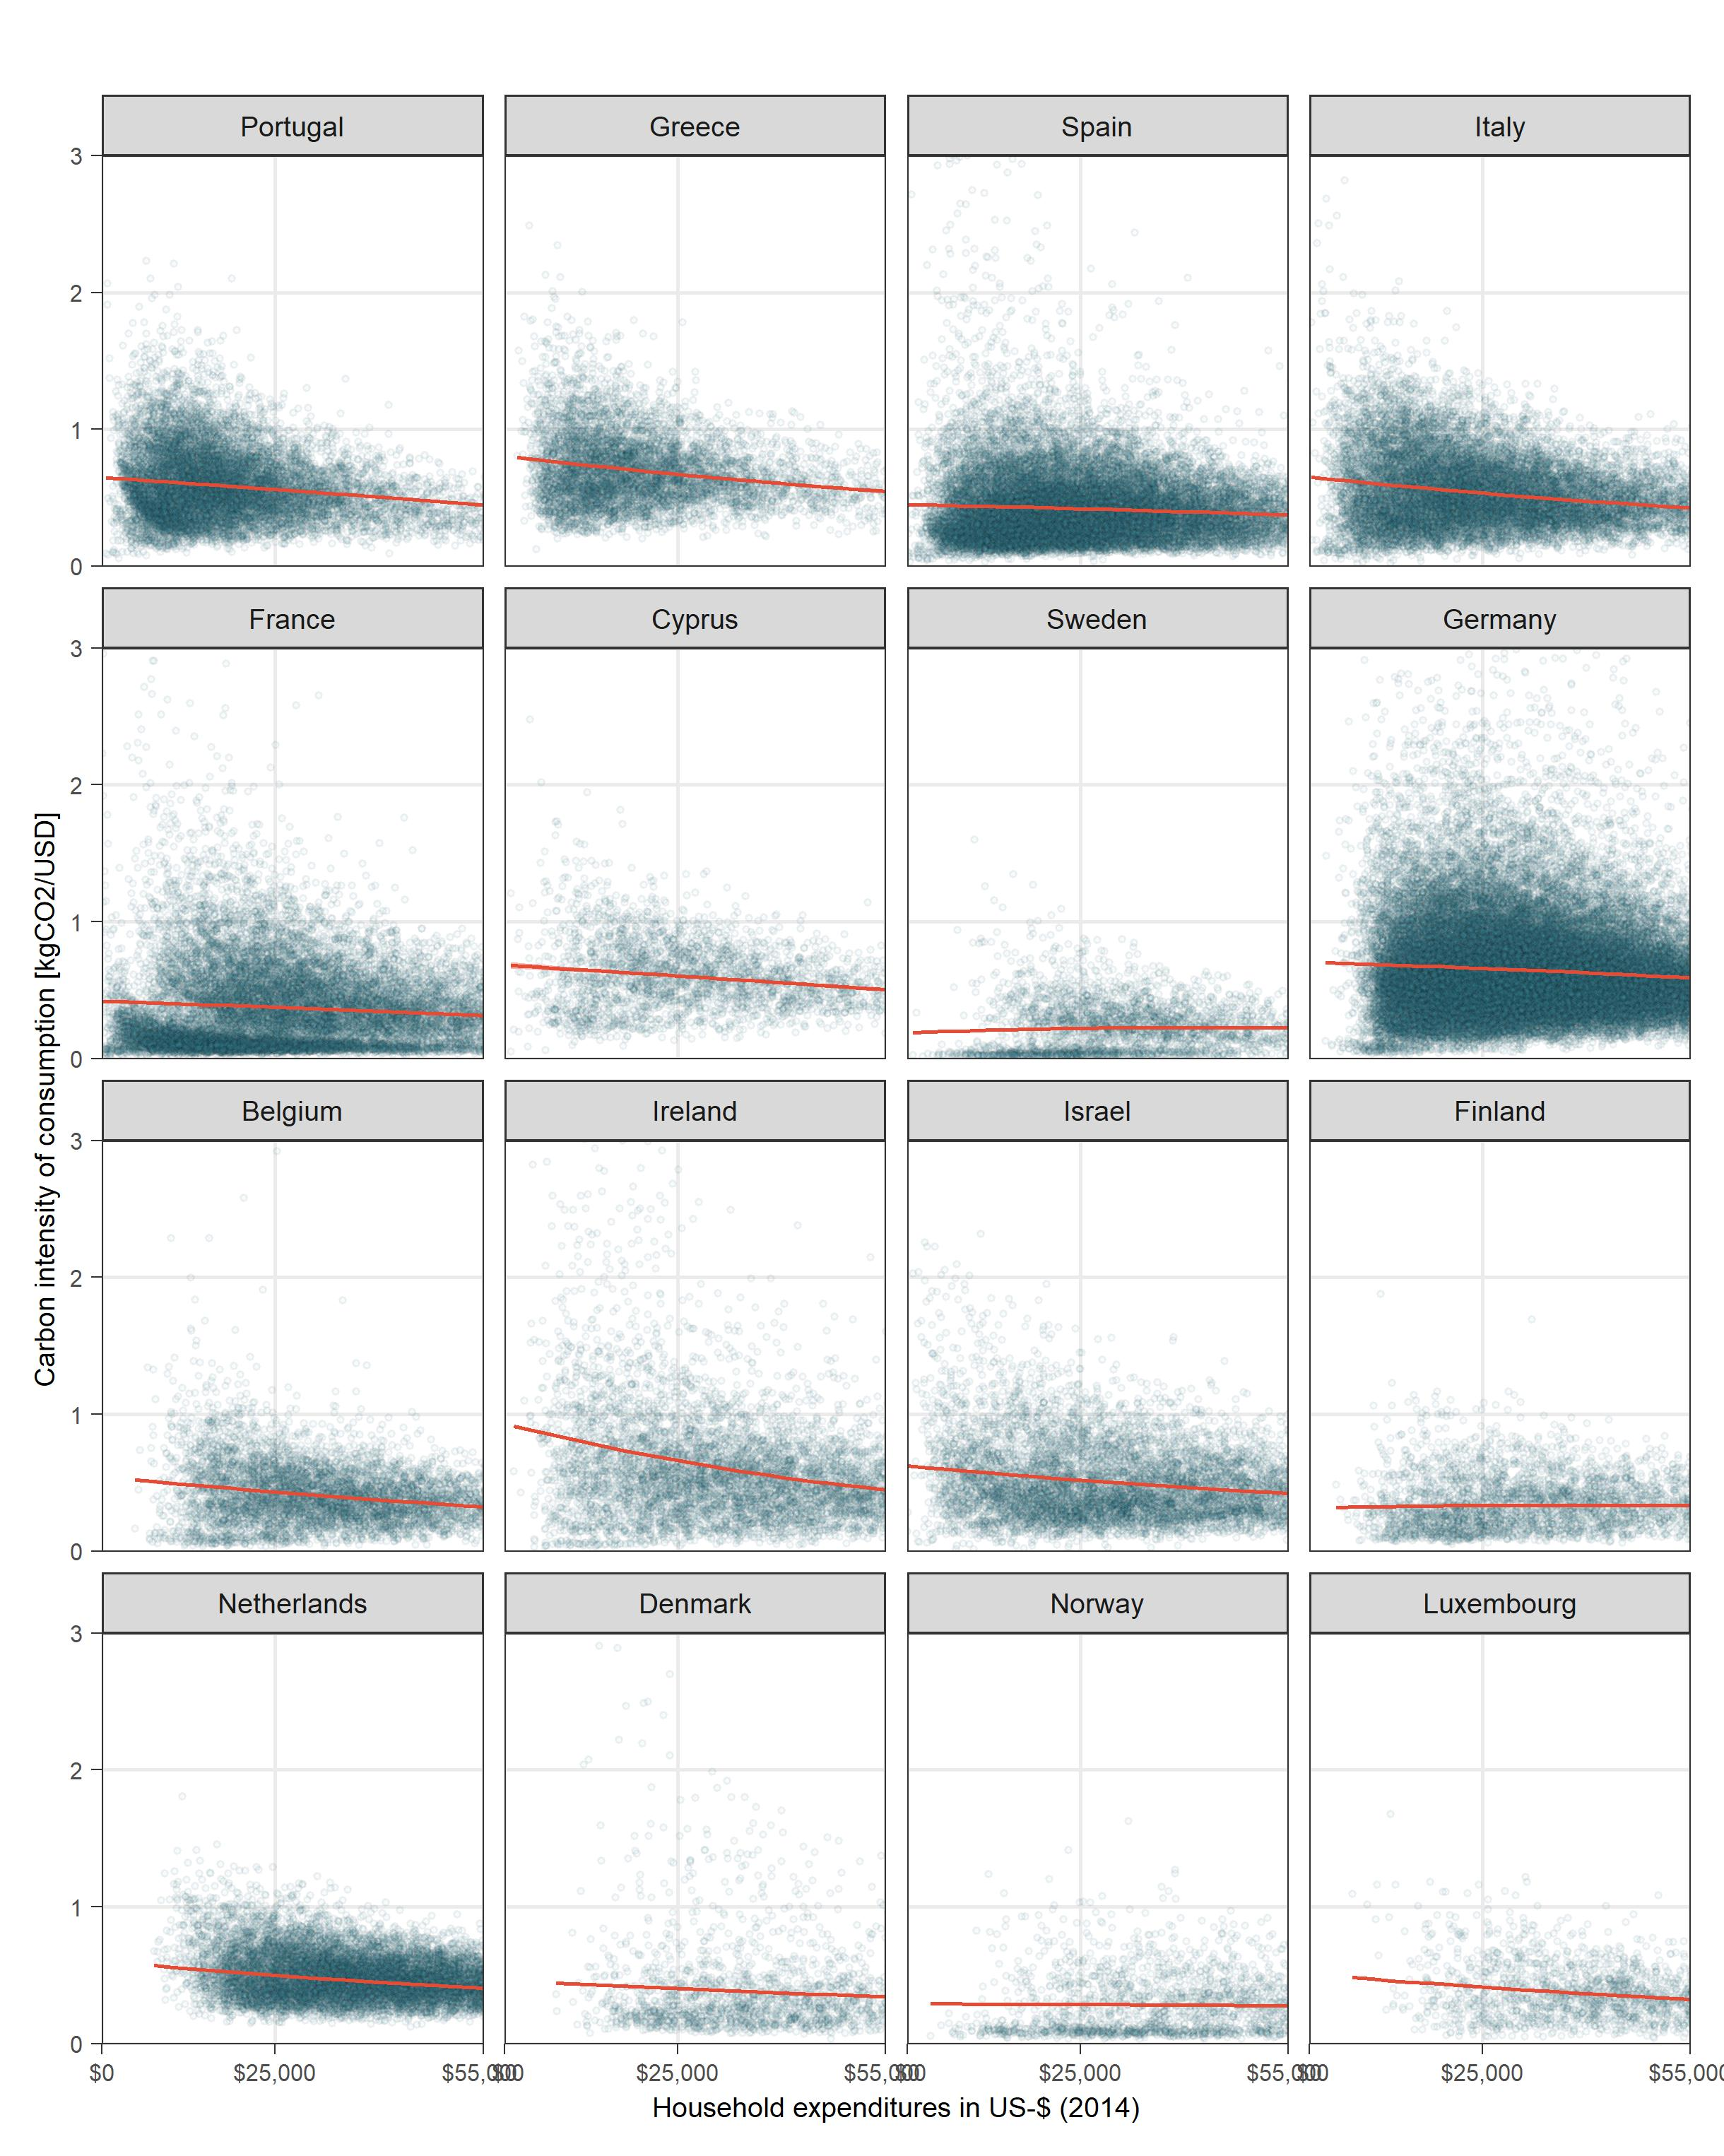
\includegraphics{Analysis_Carbon_Intensity_Curve/All_Panel_D}
  \begin{subcaption}
    This figure displays ...
  \end{subcaption}

\end{figure}

\clearpage

\subsection{Supplementary tables} \label{sec:tables}

\begin{table}[H]

\caption{Summary statistics}
\centering
\resizebox{\linewidth}{!}{
\begin{threeparttable}
\begin{tabular}[t]{>{\raggedright\arraybackslash}p{3.5 cm}|>{\raggedleft\arraybackslash}p{2.3 cm}>{\centering\arraybackslash}p{2.3 cm}>{\centering\arraybackslash}p{2.3 cm}>{\centering\arraybackslash}p{2.3 cm}>{\raggedleft\arraybackslash}p{2.3 cm}>{\centering\arraybackslash}p{2.3 cm}>{\centering\arraybackslash}p{2.3 cm}}
\toprule
Country & Observations & Average 
Household Size & Urban 
Population & Electricity 
Access & Average 
Household 
Expenditures [USD] & Car 
Ownership & Share of 
Firewood or 
 Charcoal Cons.\\
\midrule
ARG & 21,539 & 3.19 &  & 99.9\% & 14,437 & 49\% & 5\%\\
ARM & 7,776 & 3.63 & 66\% & 99.8\% & 5,371 & 32\% & 1\%\\
BEL & 6,135 & 2.31 & 96\% & NaN\% & 36,297 &  & 9\%\\
BEN & 8,012 & 5.21 & 47\% & 33.1\% & 3,127 & 3\% & 97\%\\
BFA & 7,010 & 6.51 & 31\% & 24.4\% & 3,095 & 4\% & 92\%\\
BGD & 12,240 & 4.50 & 27\% & 55.2\% & 2,125 & 1\% & 39\%\\
BGR & 2,966 & 2.37 & 71\% & NaN\% & 6,376 &  & 37\%\\
BOL & 11,859 & 3.34 & 69\% & 94.7\% & 3,688 & 17\% & 12\%\\
BRA & 57,889 & 3.01 & 86\% & 99.5\% & 12,247 & 46\% & 3\%\\
BRB & 2,434 & 2.62 &  & 94.7\% & 16,842 & 52\% & 0\%\\
CHL & 15,237 & 3.29 &  & NaN\% & 19,547 &  & 11\%\\
CIV & 12,992 & 4.48 & 52\% & 64.1\% & 3,718 & 3\% & 77\%\\
COL & 86,866 & 3.35 & 79\% & 98.3\% & 8,586 & 14\% & 9\%\\
CRI & 7,046 & 3.24 & 71\% & 99.7\% & 12,177 & 45\% & 5\%\\
CYP & 2,876 & 2.70 & 74\% & NaN\% & 31,922 &  & 21\%\\
CZE & 2,929 & 2.22 & 67\% & NaN\% & 12,615 &  & 22\%\\
DEU & 52,412 & 2.00 & 90\% & NaN\% & 32,812 &  & 0\%\\
DNK & 2,205 & 2.12 & 67\% & NaN\% & 43,812 &  & 21\%\\
DOM & 8,884 & 3.21 & 81\% & 97.5\% & 7,786 & 21\% & 7\%\\
ECU & 28,263 & 3.68 & 69\% & 90.5\% & 6,432 & 19\% & 5\%\\
ESP & 22,127 & 2.50 & 75\% & NaN\% & 26,216 &  & 0\%\\
EST & 3,395 & 2.24 & 51\% & NaN\% & 13,491 &  & 33\%\\
ETH & 6,767 & 4.48 & 32\% & 55.9\% & 1,100 & 1\% & 96\%\\
FIN & 3,673 & 2.02 & 71\% & NaN\% & 36,791 &  & 43\%\\
FRA & 16,978 & 2.23 & 69\% & NaN\% & 31,107 &  & 0\%\\
GHA & 13,521 & 3.91 & 56\% & 83.1\% & 2,312 & 4\% & 83\%\\
GNB & 5,351 & 8.18 & 47\% & 21.7\% & 4,172 & 3\% & 99\%\\
GRC & 6,150 & 2.58 & 72\% & NaN\% & 22,585 &  & 28\%\\
GTM & 11,534 & 4.77 & 54\% & 81\% & 4,830 & 17\% & 70\%\\
HRV & 2,029 & 2.89 & 59\% & NaN\% & 14,048 &  & 51\%\\
HUN & 7,185 & 2.34 & 56\% & NaN\% & 9,596 &  & 42\%\\
IDN & 295,116 & 3.77 & 55\% & 98.5\% & 2,799 & 11\% & 29\%\\
IND & 101,581 & 4.43 & 31\% & 79.9\% & 1,514 & 4\% & 63\%\\
IRL & 6,839 & 2.73 & 65\% & NaN\% & 39,751 &  & 31\%\\
IRQ & 24,994 & 6.73 & 72\% & 99.3\% & 13,940 & 35\% & 3\%\\
ISR & 8,786 & 3.28 & 90\% & NaN\% & 39,641 & 72\% & 0\%\\
ITA & 15,010 & 2.34 & 82\% & NaN\% & 27,521 &  & 15\%\\
KEN & 21,714 & 3.98 & 44\% & 56.4\% & 2,372 &  & 82\%\\
KHM & 1,206 & 4.34 & 27\% & NaN\% & 5,263 & 11\% & 73\%\\
LBR & 8,332 & 4.27 & 52\% & 16.7\% & 2,617 & 2\% & 99\%\\
LTU & 3,443 & 2.15 & 47\% & NaN\% & 10,068 &  & 33\%\\
LUX & 3,167 & 2.42 & 81\% & NaN\% & 57,666 &  & 0\%\\
LVA & 3,844 & 2.37 & 56\% & NaN\% & 11,616 &  & 0\%\\
MAR & 15,970 & 4.74 & 65\% & NaN\% & 8,194 &  & 21\%\\
MDV & 4,749 & 5.19 &  & NaN\% & 19,238 & 5\% & 0\%\\
MEX & 88,899 & 3.55 & 79\% & 99.7\% & 6,846 & 40\% & 15\%\\
MLI & 6,602 & 7.14 & 28\% & 27.5\% & 4,011 & 4\% & 99\%\\
MMR & 3,648 & 4.53 & 29\% & 63\% & 2,541 & 4\% & 88\%\\
MNG & 11,197 & 3.58 & 66\% & NaN\% & 7,174 &  & 44\%\\
MWI & 11,374 & 4.40 & 16\% & 10.7\% & 734 & 2\% & 99\%\\
NER & 6,024 & 5.96 & 17\% & 15.7\% & 2,206 & 2\% & 97\%\\
NGA & 22,110 & 5.08 & 40\% & 63.4\% & 3,955 & 8\% & 70\%\\
NIC & 6,850 & 4.38 & 60\% & 86.8\% & 4,985 & 8\% & 51\%\\
NLD & 14,408 & 2.19 & 90\% & NaN\% & 39,679 &  & 1\%\\
NOR & 3,363 & 2.77 & 82\% & NaN\% & 64,706 & 88\% & 0\%\\
PAK & 17,986 & 6.35 & 36\% & 91.5\% & 862 & 4\% & 20\%\\
PER & 34,542 & 3.56 & 77\% & 95.6\% & 4,866 & 12\% & 15\%\\
PHL & 41,540 & 4.60 & 44\% & 91.1\% & 4,838 & 7\% & 45\%\\
POL & 37,148 & 2.80 & 64\% & NaN\% & 14,962 &  & 6\%\\
PRT & 11,398 & 2.53 & 73\% & NaN\% & 20,295 &  & 9\%\\
PRY & 5,410 & 3.90 & 61\% & 97.8\% & 8,371 & 25\% & 29\%\\
ROU & 30,625 & 2.66 & 58\% & NaN\% & 6,039 &  & 9\%\\
RWA & 14,577 & 4.39 & 19\% & NaN\% & 1,353 & 1\% & 41\%\\
SEN & 7,156 & 8.91 & 53\% & 63.7\% & 7,639 & 5\% & 86\%\\
SLV & 23,622 & 3.67 & 64\% & 95.7\% & 5,707 & 15\% & 12\%\\
SUR & 2,025 & 3.39 & 72\% & NaN\% & 8,490 & 38\% & 0\%\\
SVK & 4,785 & 2.93 & 71\% & NaN\% & 15,012 &  & 19\%\\
SWE & 2,871 & 2.13 & 45\% & NaN\% & 33,704 &  & 0\%\\
TGO & 6,171 & 4.23 & 47\% & 51.8\% & 2,733 & 3\% & 92\%\\
THA & 42,711 & 3.04 & 36\% & 99.8\% & 3,917 & 14\% & 26\%\\
TUR & 10,060 & 3.64 & 70\% & NaN\% & 12,906 & 39\% & 4\%\\
UGA & 15,627 & 4.82 & 28\% & 39.2\% & 1,494 & 3\% & 95\%\\
URY & 6,888 & 2.82 & 83\% & 99.7\% & 20,528 & 46\% & 13\%\\
ZAF & 22,964 & 3.53 & 70\% & 92.7\% & 7,223 & 27\% & 10\%\\
\bottomrule
\end{tabular}
\begin{tablenotes}
\item \textit{Note: } 
\item This table provides summary statistics for households in our sample. All values (except observations) are household-weighted averages.
\end{tablenotes}
\end{threeparttable}}
\end{table}
 \label{tab:A_1}

\clearpage



\clearpage

\begin{table}[H]

\caption{Average carbon footprint and average USD/tCO$_{2}$ carbon price incidence per expenditure quintile}
\centering
\resizebox{\linewidth}{!}{
\begin{threeparttable}
\begin{tabular}[t]{l|rrrrrr|rrrrrrl|rrrrrr|rrrrrrl|rrrrrr|rrrrrrl|rrrrrr|rrrrrrl|rrrrrr|rrrrrrl|rrrrrr|rrrrrrl|rrrrrr|rrrrrrl|rrrrrr|rrrrrrl|rrrrrr|rrrrrrl|rrrrrr|rrrrrrl|rrrrrr|rrrrrrl|rrrrrr|rrrrrrl|rrrrrr|rrrrrr}
\toprule
\multicolumn{1}{c}{ } & \multicolumn{6}{c}{Average carbon footprint [tCO$_{2}$]} & \multicolumn{6}{c}{Average incidence from USD 40/tCO$_{2}$ carbon price} \\
\cmidrule(l{3pt}r{3pt}){2-7} \cmidrule(l{3pt}r{3pt}){8-13}
\multicolumn{2}{c}{ } & \multicolumn{5}{c}{Expenditure quintile} & \multicolumn{1}{c}{ } & \multicolumn{5}{c}{Expenditure quintile} \\
\cmidrule(l{3pt}r{3pt}){3-7} \cmidrule(l{3pt}r{3pt}){9-13}
Country & All & EQ1 & EQ2 & EQ3 & EQ4 & EQ5 & All & EQ1 & EQ2 & EQ3 & EQ4 & EQ5\\
\midrule
ARG & 10.4 & 5.0 & 7.7 & 9.6 & 12.8 & 16.6 & 3.19\% & 3.93\% & 3.44\% & 3.18\% & 2.93\% & 2.45\%\\
ARM & 1.2 & 0.2 & 0.3 & 0.5 & 0.7 & 4.1 & 0.92\% & 0.71\% & 0.74\% & 0.81\% & 0.89\% & 1.44\%\\
BEL & 12.9 & 11.0 & 12.9 & 13.0 & 13.2 & 14.7 & 1.58\% & 1.8\% & 1.69\% & 1.67\% & 1.49\% & 1.25\%\\
BEN & 1.3 & 0.4 & 0.7 & 1.0 & 1.4 & 3.1 & 1.47\% & 1.26\% & 1.34\% & 1.37\% & 1.43\% & 1.95\%\\
BFA & 1.9 & 0.5 & 0.9 & 1.3 & 2.1 & 4.7 & 2.16\% & 1.98\% & 2.02\% & 2.06\% & 2.17\% & 2.56\%\\
BGD & 0.9 & 0.3 & 0.4 & 0.6 & 1.0 & 1.9 & 1.48\% & 1.2\% & 1.24\% & 1.38\% & 1.63\% & 1.93\%\\
BGR & 4.7 & 2.8 & 3.4 & 4.5 & 5.7 & 7.1 & 2.94\% & 2.83\% & 2.84\% & 3.09\% & 3.05\% & 2.88\%\\
BOL & 2.3 & 1.2 & 1.9 & 2.4 & 2.8 & 3.3 & 2.64\% & 2.84\% & 2.72\% & 2.67\% & 2.62\% & 2.36\%\\
BRA & 5.7 & 1.8 & 3.1 & 4.6 & 6.7 & 12.4 & 2.17\% & 2.78\% & 2.23\% & 2.11\% & 1.98\% & 1.73\%\\
BRB & 9.9 & 4.4 & 7.6 & 10.6 & 12.0 & 14.8 & 2.49\% & 2.65\% & 2.58\% & 2.66\% & 2.5\% & 2.09\%\\
CHL & 7.9 & 4.1 & 5.8 & 7.2 & 9.2 & 13.3 & 1.85\% & 2.41\% & 2\% & 1.82\% & 1.65\% & 1.37\%\\
CIV & 1.8 & 0.8 & 1.3 & 1.7 & 2.0 & 3.0 & 1.8\% & 1.89\% & 1.84\% & 1.77\% & 1.69\% & 1.79\%\\
COL & 3.6 & 1.2 & 2.2 & 2.9 & 4.0 & 7.7 & 2.05\% & 2.52\% & 2.31\% & 2.11\% & 1.84\% & 1.46\%\\
CRI & 3.5 & 1.4 & 2.4 & 3.0 & 4.3 & 6.2 & 1.16\% & 1.14\% & 1.24\% & 1.19\% & 1.2\% & 1.04\%\\
CYP & 17.2 & 11.8 & 16.3 & 17.2 & 19.8 & 21.0 & 2.32\% & 2.61\% & 2.51\% & 2.29\% & 2.18\% & 2.01\%\\
CZE & 10.8 & 9.8 & 10.6 & 10.9 & 10.7 & 12.0 & 3.65\% & 4.11\% & 3.76\% & 3.87\% & 3.49\% & 3.03\%\\
DEU & 20.1 & 18.3 & 18.8 & 19.7 & 20.6 & 22.9 & 2.56\% & 3.04\% & 2.71\% & 2.57\% & 2.42\% & 2.06\%\\
DNK & 15.2 & 14.8 & 15.0 & 13.8 & 15.0 & 17.6 & 1.47\% & 1.73\% & 1.54\% & 1.45\% & 1.37\% & 1.25\%\\
DOM & 4.1 & 1.8 & 2.7 & 3.5 & 4.2 & 8.2 & 1.92\% & 1.78\% & 1.8\% & 1.88\% & 1.86\% & 2.29\%\\
ECU & 3.0 & 1.3 & 2.0 & 2.5 & 3.4 & 6.0 & 2.1\% & 2.57\% & 2.08\% & 1.96\% & 1.95\% & 1.92\%\\
ESP & 10.5 & 6.1 & 9.2 & 11.0 & 12.6 & 13.7 & 1.66\% & 1.8\% & 1.79\% & 1.73\% & 1.6\% & 1.41\%\\
EST & 8.5 & 4.6 & 6.5 & 8.2 & 9.4 & 13.8 & 2.72\% & 3\% & 2.95\% & 2.72\% & 2.56\% & 2.39\%\\
ETH & 0.1 & 0.0 & 0.1 & 0.1 & 0.1 & 0.2 & 0.4\% & 0.46\% & 0.4\% & 0.37\% & 0.38\% & 0.38\%\\
FIN & 12.0 & 9.4 & 10.7 & 12.2 & 12.4 & 15.3 & 1.32\% & 1.4\% & 1.36\% & 1.4\% & 1.28\% & 1.16\%\\
FRA & 10.6 & 7.9 & 10.2 & 11.4 & 11.3 & 12.1 & 1.45\% & 1.67\% & 1.56\% & 1.51\% & 1.37\% & 1.14\%\\
GHA & 0.7 & 0.3 & 0.5 & 0.7 & 1.0 & 1.3 & 1.11\% & 0.86\% & 0.99\% & 1.08\% & 1.24\% & 1.36\%\\
GNB & 1.2 & 0.3 & 0.6 & 0.9 & 1.4 & 2.9 & 0.98\% & 0.73\% & 0.76\% & 0.92\% & 1.09\% & 1.4\%\\
GRC & 14.5 & 9.9 & 12.2 & 14.0 & 15.4 & 20.8 & 2.75\% & 3.11\% & 2.94\% & 2.8\% & 2.6\% & 2.3\%\\
GTM & 2.3 & 0.5 & 1.1 & 1.8 & 2.7 & 5.2 & 1.59\% & 0.96\% & 1.22\% & 1.59\% & 1.92\% & 2.25\%\\
HRV & 8.4 & 5.0 & 7.3 & 8.2 & 9.7 & 11.8 & 2.31\% & 2.05\% & 2.4\% & 2.35\% & 2.37\% & 2.37\%\\
HUN & 6.2 & 3.9 & 5.4 & 6.3 & 7.1 & 8.1 & 2.56\% & 2.44\% & 2.64\% & 2.72\% & 2.6\% & 2.4\%\\
IDN & 2.6 & 0.9 & 1.6 & 2.3 & 3.2 & 5.2 & 3.79\% & 3.67\% & 3.62\% & 3.74\% & 3.89\% & 4.01\%\\
IND & 1.5 & 0.7 & 1.0 & 1.3 & 1.8 & 2.7 & 4.08\% & 4.2\% & 4.2\% & 4.16\% & 4.07\% & 3.77\%\\
IRL & 20.1 & 15.1 & 19.1 & 20.7 & 23.3 & 22.3 & 2.3\% & 2.79\% & 2.55\% & 2.24\% & 2.18\% & 1.72\%\\
IRQ & 8.1 & 3.9 & 5.8 & 7.4 & 9.4 & 14.0 & 2.53\% & 2.83\% & 2.63\% & 2.58\% & 2.45\% & 2.18\%\\
ISR & 17.2 & 11.8 & 15.6 & 17.6 & 19.7 & 21.4 & 1.92\% & 2.54\% & 2.08\% & 1.82\% & 1.73\% & 1.42\%\\
ITA & 13.5 & 9.1 & 12.3 & 13.5 & 15.4 & 17.3 & 2.12\% & 2.53\% & 2.28\% & 2.07\% & 1.96\% & 1.73\%\\
KEN & 1.4 & 0.3 & 0.7 & 1.1 & 1.7 & 3.5 & 2.08\% & 1.59\% & 1.92\% & 2.06\% & 2.23\% & 2.59\%\\
KHM & 1.9 & 0.8 & 1.3 & 1.6 & 2.2 & 3.5 & 1.42\% & 1.42\% & 1.52\% & 1.39\% & 1.38\% & 1.39\%\\
LBR & 0.7 & 0.1 & 0.3 & 0.6 & 1.0 & 1.6 & 0.84\% & 0.57\% & 0.68\% & 0.84\% & 0.93\% & 1.19\%\\
LTU & 3.6 & 2.1 & 2.7 & 3.2 & 4.4 & 5.4 & 1.4\% & 1.33\% & 1.37\% & 1.47\% & 1.47\% & 1.34\%\\
LUX & 17.0 & 14.7 & 15.5 & 16.9 & 18.5 & 19.2 & 1.32\% & 1.68\% & 1.42\% & 1.25\% & 1.21\% & 1.04\%\\
LVA & 6.9 & 4.4 & 5.2 & 5.9 & 7.5 & 11.3 & 2.69\% & 3.66\% & 2.81\% & 2.47\% & 2.38\% & 2.13\%\\
MAR & 3.5 & 1.9 & 2.5 & 3.0 & 3.8 & 6.3 & 1.68\% & 1.79\% & 1.67\% & 1.65\% & 1.63\% & 1.68\%\\
MDV & 7.2 & 4.8 & 6.7 & 7.4 & 8.2 & 8.7 & 1.61\% & 1.95\% & 1.8\% & 1.6\% & 1.44\% & 1.25\%\\
MEX & 4.6 & 2.0 & 3.4 & 4.4 & 5.5 & 7.6 & 2.75\% & 2.65\% & 2.79\% & 2.88\% & 2.85\% & 2.56\%\\
MLI & 1.5 & 0.5 & 0.8 & 1.2 & 1.9 & 3.0 & 1.37\% & 1.32\% & 1.34\% & 1.3\% & 1.4\% & 1.48\%\\
MMR & 1.1 & 0.4 & 0.6 & 0.9 & 1.3 & 2.4 & 1.54\% & 1.27\% & 1.41\% & 1.46\% & 1.59\% & 1.99\%\\
MNG & 11.8 & 7.1 & 9.5 & 10.9 & 12.7 & 18.9 & 7.25\% & 8.13\% & 7.82\% & 7.33\% & 6.92\% & 6.05\%\\
MWI & 0.1 & 0.0 & 0.0 & 0.1 & 0.1 & 0.4 & 0.62\% & 0.54\% & 0.52\% & 0.56\% & 0.63\% & 0.87\%\\
NER & 0.7 & 0.2 & 0.3 & 0.4 & 0.6 & 2.0 & 0.99\% & 0.9\% & 0.84\% & 0.88\% & 0.96\% & 1.38\%\\
NGA & 1.5 & 0.4 & 0.9 & 1.4 & 2.1 & 2.6 & 1.37\% & 0.96\% & 1.17\% & 1.41\% & 1.6\% & 1.71\%\\
NIC & 2.5 & 0.4 & 0.9 & 1.5 & 2.7 & 6.9 & 1.58\% & 0.99\% & 1.28\% & 1.51\% & 1.84\% & 2.25\%\\
NLD & 17.1 & 16.9 & 17.3 & 16.0 & 16.3 & 19.1 & 1.83\% & 2.16\% & 1.95\% & 1.81\% & 1.68\% & 1.53\%\\
NOR & 15.9 & 10.2 & 14.4 & 16.6 & 18.1 & 20.5 & 1.06\% & 1.11\% & 1.14\% & 1.13\% & 1.03\% & 0.88\%\\
PAK & 0.4 & 0.1 & 0.2 & 0.3 & 0.4 & 0.9 & 1.56\% & 1.26\% & 1.42\% & 1.59\% & 1.67\% & 1.85\%\\
PER & 2.2 & 1.0 & 1.8 & 2.2 & 2.6 & 3.5 & 2.16\% & 2.56\% & 2.43\% & 2.17\% & 1.95\% & 1.67\%\\
PHL & 2.2 & 0.6 & 1.1 & 1.8 & 2.8 & 4.8 & 1.64\% & 1.17\% & 1.44\% & 1.7\% & 1.9\% & 2.01\%\\
POL & 17.2 & 10.8 & 15.1 & 16.9 & 19.1 & 23.9 & 5.15\% & 5.05\% & 5.65\% & 5.67\% & 5.35\% & 4.04\%\\
PRT & 11.0 & 7.3 & 9.4 & 10.8 & 12.4 & 15.0 & 2.3\% & 2.81\% & 2.48\% & 2.3\% & 2.12\% & 1.81\%\\
PRY & 3.3 & 1.3 & 2.7 & 3.3 & 3.8 & 5.4 & 1.7\% & 1.77\% & 2.06\% & 1.75\% & 1.53\% & 1.39\%\\
ROU & 3.8 & 1.9 & 3.0 & 3.9 & 4.5 & 5.7 & 2.48\% & 1.93\% & 2.4\% & 2.63\% & 2.73\% & 2.7\%\\
RWA & 0.3 & 0.0 & 0.1 & 0.1 & 0.2 & 1.0 & 0.57\% & 0.43\% & 0.44\% & 0.5\% & 0.58\% & 0.92\%\\
SEN & 2.6 & 0.8 & 1.4 & 2.5 & 3.3 & 4.8 & 1.19\% & 0.82\% & 0.95\% & 1.23\% & 1.38\% & 1.56\%\\
SLV & 2.7 & 0.9 & 1.8 & 2.5 & 3.1 & 5.0 & 2.09\% & 2.75\% & 2.4\% & 2.04\% & 1.75\% & 1.52\%\\
SUR & 3.4 & 1.5 & 2.4 & 3.2 & 4.3 & 5.8 & 1.68\% & 1.8\% & 1.77\% & 1.7\% & 1.66\% & 1.46\%\\
SVK & 7.5 & 6.8 & 7.0 & 7.9 & 7.7 & 8.4 & 2.2\% & 2.66\% & 2.29\% & 2.36\% & 2.06\% & 1.65\%\\
SWE & 7.3 & 6.2 & 7.1 & 7.7 & 7.1 & 8.5 & 0.88\% & 0.99\% & 0.92\% & 0.9\% & 0.78\% & 0.78\%\\
TGO & 0.9 & 0.2 & 0.5 & 0.7 & 1.1 & 1.8 & 1.06\% & 0.76\% & 0.98\% & 1.01\% & 1.13\% & 1.41\%\\
THA & 3.8 & 1.2 & 2.2 & 3.5 & 5.0 & 7.2 & 4.06\% & 4.06\% & 4.47\% & 4.46\% & 3.96\% & 3.36\%\\
TUR & 11.5 & 7.2 & 10.2 & 11.8 & 12.7 & 15.5 & 4.04\% & 4.43\% & 4.74\% & 4.32\% & 3.76\% & 2.97\%\\
UGA & 0.4 & 0.1 & 0.1 & 0.2 & 0.4 & 1.1 & 0.91\% & 1.03\% & 0.75\% & 0.74\% & 0.83\% & 1.2\%\\
URY & 3.7 & 1.8 & 2.6 & 3.4 & 4.5 & 6.4 & 0.78\% & 0.92\% & 0.81\% & 0.77\% & 0.72\% & 0.66\%\\
ZAF & 13.0 & 4.0 & 6.2 & 8.5 & 14.0 & 32.3 & 8.51\% & 9.67\% & 8.79\% & 8.67\% & 8.36\% & 7.03\%\\
\bottomrule
\end{tabular}
\begin{tablenotes}
\item \textit{Note: } 
\item This table shows average carbon footprints in tCO$_{2}$ and average levels of carbon price incidence for households in all countries of our sample. We estimate household-weighted averages for the whole population and per expenditure quintile.
\end{tablenotes}
\end{threeparttable}}
\end{table}
 \label{tab:A3}

\clearpage

\begin{table}[H]

\caption{\label{tab:A4_CF}Share of households using cooking fuels}
\centering
\resizebox{\linewidth}{!}{
\begin{threeparttable}
\begin{tabular}[t]{l|rrrrr|rrrrr|rrrrrl|rrrrr|rrrrr|rrrrrl|rrrrr|rrrrr|rrrrrl|rrrrr|rrrrr|rrrrrl|rrrrr|rrrrr|rrrrrl|rrrrr|rrrrr|rrrrrl|rrrrr|rrrrr|rrrrrl|rrrrr|rrrrr|rrrrrl|rrrrr|rrrrr|rrrrrl|rrrrr|rrrrr|rrrrrl|rrrrr|rrrrr|rrrrrl|rrrrr|rrrrr|rrrrrl|rrrrr|rrrrr|rrrrrl|rrrrr|rrrrr|rrrrrl|rrrrr|rrrrr|rrrrrl|rrrrr|rrrrr|rrrrr}
\toprule
\multicolumn{1}{c}{ } & \multicolumn{5}{c}{Solid fuels} & \multicolumn{5}{c}{Liquid or gaseous fuels} & \multicolumn{5}{c}{Electricity} \\
\cmidrule(l{3pt}r{3pt}){2-6} \cmidrule(l{3pt}r{3pt}){7-11} \cmidrule(l{3pt}r{3pt}){12-16}
\multicolumn{1}{c}{ } & \multicolumn{5}{c}{Expenditure quintile} & \multicolumn{5}{c}{Expenditure quintile} & \multicolumn{5}{c}{Expenditure quintile} \\
\cmidrule(l{3pt}r{3pt}){2-6} \cmidrule(l{3pt}r{3pt}){7-11} \cmidrule(l{3pt}r{3pt}){12-16}
Country & EQ1 & EQG2 & EQ3 & EQ4 & EQ5 & EQ1 & EQG2 & EQ3 & EQ4 & EQ5 & EQ1 & EQG2 & EQ3 & EQ4 & EQ5\\
\midrule
Argentina & - & - & - & - & - & 99\% & 99\% & 99\% & 98\% & 96\% & 1\% & 0\% & 1\% & 2\% & 4\%\\
Barbados & 0\% & 0\% & - & - & - & 89\% & 95\% & 94\% & 94\% & 88\% & 4\% & 4\% & 5\% & 5\% & 11\%\\
Benin & 100\% & 100\% & 99\% & 96\% & 77\% & - & 0\% & 1\% & 3\% & 23\% & - & - & - & - & -\\
Bolivia & 36\% & 12\% & 6\% & 3\% & 2\% & 63\% & 87\% & 92\% & 93\% & 89\% & - & 0\% & 0\% & 0\% & 1\%\\
Brazil & 3\% & 1\% & 0\% & 0\% & 0\% & 95\% & 98\% & 98\% & 99\% & 98\% & 0\% & 1\% & 1\% & 1\% & 1\%\\
Burkina Faso & 99\% & 100\% & 98\% & 89\% & 43\% & 0\% & 0\% & 1\% & 11\% & 56\% & - & - & - & - & -\\
Cambodia & 82\% & 59\% & 59\% & 44\% & 24\% & 17\% & 41\% & 41\% & 54\% & 74\% & 1\% & 0\% & 1\% & 0\% & 2\%\\
Colombia & 28\% & 10\% & 4\% & 3\% & 1\% & 68\% & 86\% & 92\% & 92\% & 92\% & 3\% & 3\% & 3\% & 3\% & 5\%\\
Costa Rica & 11\% & 4\% & 3\% & 2\% & 1\% & 52\% & 54\% & 47\% & 44\% & 29\% & 36\% & 41\% & 50\% & 54\% & 69\%\\
Côte d’Ivoire & 97\% & 92\% & 73\% & 49\% & 27\% & 2\% & 8\% & 26\% & 49\% & 68\% & - & - & - & - & 0\%\\
Dominican Republic & 10\% & 4\% & 3\% & 2\% & 1\% & 89\% & 94\% & 93\% & 92\% & 91\% & 0\% & - & 0\% & 0\% & 0\%\\
Ecuador & 15\% & 4\% & 2\% & 1\% & 0\% & 80\% & 94\% & 95\% & 96\% & 95\% & 0\% & 0\% & 0\% & 0\% & 1\%\\
Egypt & 0\% & 0\% & 0\% & 0\% & - & 100\% & 100\% & 100\% & 100\% & 100\% & 0\% & 0\% & - & 0\% & 0\%\\
El Salvador & 32\% & 12\% & 7\% & 3\% & 2\% & 62\% & 87\% & 91\% & 95\% & 88\% & 0\% & 0\% & 1\% & 1\% & 4\%\\
Ethiopia & 99\% & 99\% & 98\% & 90\% & 64\% & 0\% & 1\% & 0\% & 1\% & 2\% & 0\% & 0\% & 1\% & 8\% & 29\%\\
Georgia & - & - & - & - & - & 95\% & 97\% & 98\% & 98\% & 99\% & - & - & - & - & -\\
Ghana & 97\% & 87\% & 70\% & 55\% & 31\% & 2\% & 11\% & 25\% & 35\% & 51\% & - & 0\% & 0\% & 0\% & 1\%\\
Guatemala & 98\% & 92\% & 75\% & 58\% & 28\% & 1\% & 7\% & 23\% & 41\% & 68\% & - & - & - & - & -\\
Guinea-Bissau & 100\% & 99\% & 98\% & 99\% & 93\% & - & 0\% & 0\% & 1\% & 6\% & - & - & - & - & -\\
India & 92\% & 84\% & 70\% & 41\% & 9\% & 2\% & 9\% & 25\% & 56\% & 79\% & 0\% & 0\% & 0\% & 0\% & 0\%\\
Indonesia & 42\% & 21\% & 12\% & 6\% & 2\% & 57\% & 78\% & 87\% & 92\% & 92\% & 0\% & 0\% & 0\% & 1\% & 1\%\\
Iraq & 2\% & 0\% & 0\% & 0\% & 0\% & 98\% & 99\% & 100\% & 99\% & 99\% & 1\% & 1\% & 0\% & 1\% & 0\%\\
Jordan & 0\% & 0\% & 0\% & - & - & 100\% & 100\% & 100\% & 100\% & 100\% & - & - & - & - & -\\
Kenya & 98\% & 94\% & 79\% & 52\% & 24\% & 1\% & 5\% & 18\% & 44\% & 70\% & 0\% & 0\% & 1\% & 2\% & 2\%\\
Liberia & 100\% & 99\% & 99\% & 99\% & 98\% & 0\% & 0\% & - & 0\% & 0\% & 0\% & - & - & 0\% & 0\%\\
Malawi & 100\% & 100\% & 100\% & 100\% & 95\% & - & - & - & - & - & - & - & 0\% & 0\% & 5\%\\
Maldives & 2\% & 0\% & 0\% & - & - & 96\% & 96\% & 98\% & 97\% & 95\% & 0\% & 1\% & 1\% & 1\% & 2\%\\
Mali & 100\% & 100\% & 100\% & 99\% & 94\% & - & - & - & 1\% & 5\% & - & - & - & - & -\\
Mexico & 43\% & 17\% & 9\% & 4\% & 2\% & 56\% & 81\% & 90\% & 94\% & 95\% & 1\% & 1\% & 1\% & 1\% & 2\%\\
Mozambique & 100\% & 100\% & 99\% & 99\% & 85\% & 0\% & 0\% & 0\% & 1\% & 11\% & - & 0\% & 0\% & 1\% & 4\%\\
Myanmar (Burma) & 95\% & 90\% & 85\% & 78\% & 66\% & 1\% & 0\% & 1\% & 1\% & 3\% & 3\% & 10\% & 14\% & 19\% & 30\%\\
Nicaragua & 94\% & 75\% & 49\% & 28\% & 10\% & 5\% & 24\% & 50\% & 70\% & 88\% & 0\% & 0\% & 1\% & 1\% & 0\%\\
Niger & 98\% & 99\% & 99\% & 98\% & 81\% & - & - & 0\% & 1\% & 18\% & - & - & - & - & -\\
Nigeria & 98\% & 91\% & 72\% & 47\% & 19\% & 1\% & 9\% & 27\% & 52\% & 77\% & - & - & - & - & -\\
Paraguay & 83\% & 56\% & 28\% & 17\% & 5\% & 12\% & 38\% & 65\% & 74\% & 81\% & 2\% & 4\% & 5\% & 8\% & 10\%\\
Peru & 31\% & 10\% & 4\% & 2\% & 0\% & 60\% & 85\% & 89\% & 87\% & 76\% & 1\% & 3\% & 5\% & 11\% & 21\%\\
Rwanda & - & - & - & - & 0\% & - & - & - & 0\% & 5\% & 99\% & 99\% & 99\% & 100\% & 94\%\\
Senegal & 98\% & 90\% & 71\% & 48\% & 18\% & 2\% & 10\% & 29\% & 51\% & 79\% & - & - & - & 0\% & 0\%\\
South Africa & 28\% & 13\% & 6\% & 2\% & 0\% & 8\% & 9\% & 9\% & 6\% & 8\% & 63\% & 77\% & 85\% & 91\% & 92\%\\
Suriname & - & - & - & - & - & 99\% & 98\% & 99\% & 97\% & 96\% & 0\% & 2\% & 0\% & 2\% & 2\%\\
Thailand & 56\% & 33\% & 16\% & 8\% & 4\% & 38\% & 63\% & 77\% & 76\% & 67\% & 1\% & 1\% & 2\% & 4\% & 7\%\\
Togo & 100\% & 99\% & 96\% & 90\% & 62\% & - & 0\% & 3\% & 9\% & 36\% & - & - & - & - & -\\
Turkey & 16\% & 3\% & 1\% & 1\% & 0\% & 80\% & 96\% & 98\% & 98\% & 98\% & 3\% & 1\% & 0\% & 1\% & 2\%\\
Uganda & 96\% & 98\% & 97\% & 95\% & 85\% & 0\% & 0\% & 0\% & 1\% & 6\% & 0\% & 0\% & 0\% & 1\% & 2\%\\
Uruguay & 3\% & 1\% & 1\% & 1\% & 0\% & 93\% & 96\% & 96\% & 94\% & 90\% & 3\% & 3\% & 3\% & 6\% & 10\%\\
\bottomrule
\end{tabular}
\begin{tablenotes}
\item \textit{Note: } 
\item This table shows the share of households using different cooking fuels, such as solid fuels (e.g., firewood, charcoal, coal, biomass), liquid fuels (e.g., LPG, natural gas, kerosene), or electricity over expenditure quintiles.
\end{tablenotes}
\end{threeparttable}}
\end{table}
 \label{tab:A4_CF}

\begin{table}[H]

\caption{Share of households using lighting fuels}
\centering
\resizebox{\linewidth}{!}{
\begin{threeparttable}
\begin{tabular}[t]{l|rrrrr|rrrrr|rrrrrl|rrrrr|rrrrr|rrrrrl|rrrrr|rrrrr|rrrrrl|rrrrr|rrrrr|rrrrrl|rrrrr|rrrrr|rrrrrl|rrrrr|rrrrr|rrrrrl|rrrrr|rrrrr|rrrrrl|rrrrr|rrrrr|rrrrrl|rrrrr|rrrrr|rrrrrl|rrrrr|rrrrr|rrrrrl|rrrrr|rrrrr|rrrrrl|rrrrr|rrrrr|rrrrrl|rrrrr|rrrrr|rrrrrl|rrrrr|rrrrr|rrrrrl|rrrrr|rrrrr|rrrrrl|rrrrr|rrrrr|rrrrr}
\toprule
\multicolumn{1}{c}{ } & \multicolumn{5}{c}{Kerosene} & \multicolumn{5}{c}{Electricity} & \multicolumn{5}{c}{Other lighting fuels} \\
\cmidrule(l{3pt}r{3pt}){2-6} \cmidrule(l{3pt}r{3pt}){7-11} \cmidrule(l{3pt}r{3pt}){12-16}
\multicolumn{1}{c}{ } & \multicolumn{5}{c}{Expenditure quintile} & \multicolumn{5}{c}{Expenditure quintile} & \multicolumn{5}{c}{Expenditure quintile} \\
\cmidrule(l{3pt}r{3pt}){2-6} \cmidrule(l{3pt}r{3pt}){7-11} \cmidrule(l{3pt}r{3pt}){12-16}
Country & EQ1 & EQ2 & EQ3 & EQ4 & EQ5 & EQ1 & EQ2 & EQ3 & EQ4 & EQ5 & EQ1 & EQ2 & EQ3 & EQ4 & EQ5\\
\midrule
BEN & 1\% & 0\% & 1\% & 0\% & 1\% & 20\% & 30\% & 42\% & 60\% & 74\% & 80\% & 70\% & 58\% & 40\% & 25\%\\
BFA & 0\% & 0\% & 0\% & 0\% & 0\% & 29\% & 38\% & 44\% & 66\% & 91\% & 65\% & 59\% & 52\% & 30\% & 8\%\\
BRB & 1\% & 1\% & 1\% & 0\% & - & 88\% & 95\% & 97\% & 97\% & 97\% & 3\% & 3\% & 2\% & 2\% & 1\%\\
CIV & 0\% & 0\% & 0\% & 0\% & 0\% & 60\% & 74\% & 84\% & 90\% & 95\% & 37\% & 24\% & 15\% & 9\% & 4\%\\
CRI & - & - & - & - & - & 99\% & 100\% & 100\% & 100\% & 100\% & - & - & - & - & -\\
DOM & 2\% & 2\% & 1\% & 1\% & 0\% & 96\% & 97\% & 98\% & 98\% & 99\% & 2\% & 1\% & 1\% & 1\% & 0\%\\
ECU & - & - & - & - & - & 95\% & 99\% & 99\% & 100\% & 100\% & - & - & - & - & -\\
ETH & 30\% & 27\% & 23\% & 14\% & 3\% & 30\% & 43\% & 48\% & 68\% & 90\% & 41\% & 29\% & 29\% & 18\% & 7\%\\
GHA & 1\% & 1\% & 1\% & 1\% & - & - & - & - & - & - & 36\% & 17\% & 11\% & 7\% & 4\%\\
GNB & 1\% & 0\% & 0\% & 0\% & 0\% & 43\% & 46\% & 49\% & 58\% & 72\% & 48\% & 48\% & 47\% & 37\% & 25\%\\
GTM & - & - & - & - & - & 58\% & 82\% & 89\% & 96\% & 97\% & 37\% & 15\% & 9\% & 4\% & 2\%\\
IDN & - & - & - & - & - & 96\% & 98\% & 99\% & 100\% & 100\% & - & - & - & - & -\\
IND & 48\% & 28\% & 15\% & 6\% & 2\% & 51\% & 72\% & 85\% & 94\% & 98\% & 0\% & 0\% & 0\% & 0\% & 0\%\\
IRQ & 1\% & 0\% & 0\% & 0\% & 0\% & 99\% & 100\% & 100\% & 100\% & 100\% & 0\% & - & - & - & -\\
KEN & 56\% & 53\% & 37\% & 20\% & 9\% & 23\% & 38\% & 57\% & 75\% & 88\% & 18\% & 8\% & 5\% & 4\% & 2\%\\
KHM & 2\% & 1\% & - & - & 1\% & 85\% & 95\% & 96\% & 96\% & 98\% & 13\% & 5\% & 4\% & 4\% & 1\%\\
LBR & - & 0\% & 0\% & - & - & 0\% & 3\% & 9\% & 20\% & 40\% & 98\% & 96\% & 90\% & 79\% & 57\%\\
MLI & 1\% & 1\% & 0\% & 0\% & 0\% & 61\% & 66\% & 68\% & 80\% & 94\% & 27\% & 26\% & 26\% & 18\% & 5\%\\
MMR & 13\% & 5\% & 4\% & 5\% & 2\% & 46\% & 55\% & 61\% & 69\% & 77\% & 41\% & 39\% & 35\% & 27\% & 21\%\\
MWI & 1\% & 1\% & 0\% & 0\% & 0\% & 0\% & 1\% & 3\% & 10\% & 41\% & 97\% & 97\% & 95\% & 88\% & 57\%\\
NER & 1\% & 0\% & 0\% & 0\% & 0\% & 3\% & 6\% & 13\% & 25\% & 58\% & 95\% & 94\% & 87\% & 74\% & 41\%\\
NIC & 13\% & 4\% & 3\% & 2\% & 0\% & 62\% & 85\% & 92\% & 96\% & 99\% & - & - & - & - & -\\
PER & 1\% & 0\% & 0\% & 0\% & 0\% & 86\% & 96\% & 98\% & 99\% & 99\% & - & - & - & - & -\\
RWA & - & - & - & - & - & 79\% & 83\% & 83\% & 85\% & 92\% & 20\% & 16\% & 16\% & 14\% & 8\%\\
SEN & 1\% & 1\% & 0\% & 0\% & 0\% & 40\% & 61\% & 83\% & 91\% & 96\% & 55\% & 35\% & 14\% & 8\% & 3\%\\
SLV & 4\% & 1\% & 0\% & 0\% & 0\% & 87\% & 96\% & 98\% & 99\% & 99\% & - & - & - & - & -\\
SUR & - & - & - & - & - & 89\% & 96\% & 99\% & 99\% & 99\% & 6\% & 2\% & 1\% & 0\% & 1\%\\
TGO & 0\% & 0\% & 1\% & 0\% & 0\% & 13\% & 36\% & 62\% & 79\% & 89\% & 85\% & 63\% & 37\% & 19\% & 10\%\\
UGA & 44\% & 50\% & 40\% & 24\% & 10\% & 14\% & 21\% & 33\% & 52\% & 76\% & 8\% & 3\% & 3\% & 5\% & 4\%\\
URY & 0\% & 0\% & - & - & - & 99\% & 100\% & 100\% & 100\% & 100\% & 1\% & 0\% & 0\% & 0\% & 0\%\\
ZAF & 3\% & 2\% & 2\% & 1\% & 0\% & 85\% & 89\% & 92\% & 96\% & 99\% & 12\% & 8\% & 6\% & 3\% & 0\%\\
\bottomrule
\end{tabular}
\begin{tablenotes}
\item \textit{Note: } 
\item This table shows the share of households using different lighting fuels over expenditure quintiles.
\end{tablenotes}
\end{threeparttable}}
\end{table}
 \label{tab:A4_LF}

\begin{table}[H]

\caption{\label{tab:A6}Share of households possessing different assets}
\centering
\resizebox{\linewidth}{!}{
\begin{threeparttable}
\begin{tabular}[t]{l|rrr|rrr|rrr|rrr|rrrl|rrr|rrr|rrr|rrr|rrrl|rrr|rrr|rrr|rrr|rrrl|rrr|rrr|rrr|rrr|rrrl|rrr|rrr|rrr|rrr|rrrl|rrr|rrr|rrr|rrr|rrrl|rrr|rrr|rrr|rrr|rrrl|rrr|rrr|rrr|rrr|rrrl|rrr|rrr|rrr|rrr|rrrl|rrr|rrr|rrr|rrr|rrrl|rrr|rrr|rrr|rrr|rrrl|rrr|rrr|rrr|rrr|rrrl|rrr|rrr|rrr|rrr|rrrl|rrr|rrr|rrr|rrr|rrrl|rrr|rrr|rrr|rrr|rrrl|rrr|rrr|rrr|rrr|rrr}
\toprule
\multicolumn{1}{c}{ } & \multicolumn{3}{c}{Car} & \multicolumn{3}{c}{TV} & \multicolumn{3}{c}{Refrigerator} & \multicolumn{3}{c}{AC} & \multicolumn{3}{c}{Washing machine} \\
\cmidrule(l{3pt}r{3pt}){2-4} \cmidrule(l{3pt}r{3pt}){5-7} \cmidrule(l{3pt}r{3pt}){8-10} \cmidrule(l{3pt}r{3pt}){11-13} \cmidrule(l{3pt}r{3pt}){14-16}
Country & All & EQ1 & EQ5 & All & EQ1 & EQ5 & All & EQ1 & EQ5 & All & EQ1 & EQ5 & All & EQ1 & EQ5\\
\midrule
ARG & 49\% & 26\% & 66\% & 97\% & 96\% & 97\% & 98\% & 95\% & 99\% & 53\% & 33\% & 72\% & 87\% & 81\% & 87\%\\
ARM & 32\% & 24\% & 41\% & 99\% & 99\% & 99\% & 96\% & 94\% & 98\% & 8\% & 4\% & 14\% & 92\% & 91\% & 95\%\\
AUT & 77\% & 70\% & 82\% & 94\% & 94\% & 93\% & 99\% & 99\% & 99\% & 4\% & 2\% & 6\% & 95\% & 95\% & 95\%\\
BEN & 3\% & 0\% & 12\% & 23\% & 3\% & 52\% & 4\% & 0\% & 14\% & 0\% & 0\% & 1\% & 0\% & 0\% & 1\%\\
BFA & 4\% & 0\% & 17\% & 30\% & 3\% & 78\% & 9\% & 0\% & 38\% & 2\% & 0\% & 8\% & 0\% & 0\% & 0\%\\
BGD & 1\% & 0\% & 2\% & 36\% & 9\% & 71\% & 12\% & 0\% & 44\% & - & - & - & 0\% & 0\% & 1\%\\
BOL & 17\% & 5\% & 31\% & 84\% & 61\% & 92\% & 61\% & 28\% & 77\% & 10\% & 2\% & 22\% & 18\% & 2\% & 40\%\\
BRA & 46\% & 17\% & 77\% & 97\% & 94\% & 98\% & 98\% & 96\% & 99\% & 20\% & 6\% & 42\% & 65\% & 37\% & 87\%\\
BRB & 52\% & 21\% & 75\% & 49\% & 34\% & 61\% & 94\% & 84\% & 97\% & 8\% & 2\% & 18\% & 75\% & 60\% & 86\%\\
CAN & 86\% & 74\% & 94\% & 74\% & 75\% & 72\% & - & - & - & - & - & - & - & - & -\\
CHE & 77\% & 79\% & 80\% & 92\% & 92\% & 91\% & 64\% & 73\% & 54\% & - & - & - & 59\% & 60\% & 58\%\\
CIV & 3\% & 0\% & 10\% & 45\% & 15\% & 70\% & 15\% & 1\% & 35\% & 2\% & 0\% & 9\% & 2\% & 1\% & 5\%\\
COL & 14\% & 1\% & 39\% & 92\% & 81\% & 97\% & 83\% & 66\% & 92\% & 4\% & 1\% & 7\% & 61\% & 34\% & 82\%\\
CRI & 45\% & 19\% & 74\% & 97\% & 95\% & 98\% & 96\% & 92\% & 98\% & - & - & - & - & - & -\\
DOM & 21\% & 6\% & 45\% & 87\% & 83\% & 89\% & 83\% & 74\% & 87\% & 14\% & 2\% & 37\% & 80\% & 72\% & 84\%\\
ECU & 19\% & 2\% & 52\% & 91\% & 78\% & 98\% & 80\% & 56\% & 93\% & 6\% & 0\% & 17\% & 45\% & 15\% & 71\%\\
EGY & 7\% & 1\% & 21\% & 96\% & 95\% & 97\% & 97\% & 95\% & 98\% & 12\% & 4\% & 29\% & 95\% & 95\% & 94\%\\
ETH & 1\% & 0\% & 4\% & 18\% & 1\% & 51\% & 7\% & 0\% & 25\% & - & - & - & - & - & -\\
GBR & 75\% & 53\% & 87\% & 97\% & 97\% & 97\% & 98\% & 98\% & 98\% & - & - & - & 98\% & 97\% & 99\%\\
GEO & 29\% & 18\% & 37\% & 96\% & 94\% & 95\% & 91\% & 85\% & 93\% & 8\% & 1\% & 17\% & 74\% & 61\% & 83\%\\
GHA & 4\% & 1\% & 9\% & 64\% & 31\% & 85\% & 36\% & 7\% & 57\% & 1\% & 0\% & 3\% & 1\% & 0\% & 3\%\\
GNB & 3\% & 0\% & 12\% & 26\% & 5\% & 59\% & 13\% & 0\% & 40\% & 1\% & 0\% & 2\% & 0\% & 0\% & 1\%\\
GTM & 17\% & 2\% & 44\% & 71\% & 34\% & 92\% & 5\% & 0\% & 16\% & - & - & - & 11\% & 0\% & 36\%\\
IDN & 11\% & 1\% & 36\% & 14\% & 2\% & 38\% & 57\% & 25\% & 80\% & 8\% & 0\% & 29\% & - & - & -\\
IND & 4\% & 1\% & 15\% & 59\% & 23\% & 82\% & 20\% & 1\% & 58\% & 12\% & 2\% & 30\% & 9\% & 0\% & 32\%\\
IRQ & 35\% & 17\% & 62\% & - & - & - & 92\% & 83\% & 98\% & 41\% & 21\% & 59\% & 69\% & 41\% & 89\%\\
ISR & 72\% & 53\% & 82\% & 88\% & 76\% & 93\% & 100\% & 100\% & 100\% & 93\% & 89\% & 97\% & 96\% & 97\% & 94\%\\
JOR & 51\% & 27\% & 70\% & 99\% & 98\% & 100\% & 98\% & 96\% & 98\% & 20\% & 9\% & 39\% & 97\% & 95\% & 97\%\\
KHM & 11\% & 2\% & 34\% & - & - & - & - & - & - & - & - & - & - & - & -\\
LBR & 2\% & 0\% & 6\% & 18\% & 1\% & 43\% & 4\% & 0\% & 15\% & 0\% & 0\% & 1\% & - & - & -\\
MDV & 5\% & 2\% & 8\% & 87\% & 86\% & 81\% & 90\% & 92\% & 82\% & 68\% & 58\% & 65\% & 90\% & 92\% & 82\%\\
MEX & 38\% & 17\% & 58\% & 71\% & 75\% & 58\% & 86\% & 70\% & 94\% & 15\% & 6\% & 27\% & 68\% & 46\% & 82\%\\
MLI & 4\% & 0\% & 17\% & 37\% & 13\% & 73\% & 10\% & 0\% & 34\% & 2\% & 0\% & 10\% & 0\% & 0\% & 0\%\\
MMR & 4\% & 0\% & 11\% & 49\% & 26\% & 72\% & 14\% & 1\% & 34\% & 3\% & 0\% & 11\% & 4\% & 0\% & 12\%\\
MNG & - & - & - & 97\% & 94\% & 99\% & - & - & - & - & - & - & - & - & -\\
MOZ & 1\% & 0\% & 3\% & 4\% & 0\% & 11\% & 2\% & 0\% & 8\% & 0\% & 0\% & 0\% & 0\% & 0\% & 0\%\\
MWI & 2\% & 0\% & 6\% & 11\% & 0\% & 38\% & 4\% & 0\% & 19\% & 0\% & 0\% & 0\% & 0\% & 0\% & 0\%\\
NER & 2\% & 0\% & 9\% & 10\% & 0\% & 41\% & 4\% & 0\% & 18\% & 1\% & 0\% & 4\% & 0\% & 0\% & 0\%\\
NGA & 8\% & 1\% & 19\% & 48\% & 11\% & 76\% & 24\% & 2\% & 49\% & 3\% & 0\% & 9\% & 2\% & 0\% & 8\%\\
NIC & 8\% & 0\% & 29\% & 75\% & 39\% & 95\% & 40\% & 7\% & 79\% & 1\% & 0\% & 6\% & 10\% & 0\% & 31\%\\
NOR & 88\% & 85\% & 93\% & 97\% & 96\% & 98\% & 96\% & 96\% & 97\% & - & - & - & 94\% & 93\% & 96\%\\
PER & 12\% & 2\% & 29\% & 81\% & 52\% & 93\% & 53\% & 15\% & 80\% & - & - & - & 30\% & 3\% & 61\%\\
PHL & 7\% & 0\% & 27\% & 77\% & 45\% & 95\% & 41\% & 6\% & 81\% & 12\% & 0\% & 40\% & 36\% & 4\% & 72\%\\
PRY & 25\% & 2\% & 57\% & 87\% & 71\% & 93\% & 80\% & 59\% & 90\% & 25\% & 2\% & 60\% & 66\% & 40\% & 77\%\\
RUS & 41\% & 33\% & 45\% & 98\% & 98\% & 98\% & 64\% & 55\% & 70\% & 9\% & 7\% & 11\% & 79\% & 70\% & 82\%\\
RWA & 1\% & 0\% & 5\% & 10\% & 0\% & 37\% & 2\% & 0\% & 8\% & - & - & - & 0\% & 0\% & 0\%\\
SEN & 5\% & 0\% & 20\% & 58\% & 17\% & 85\% & 32\% & 4\% & 65\% & 2\% & 0\% & 11\% & 0\% & 0\% & 2\%\\
SLV & 15\% & 1\% & 40\% & 87\% & 68\% & 95\% & 67\% & 36\% & 84\% & 1\% & 0\% & 5\% & 17\% & 2\% & 44\%\\
SRB & 91\% & 87\% & 95\% & 38\% & 13\% & 60\% & 76\% & 80\% & 70\% & 19\% & 8\% & 31\% & 45\% & 29\% & 62\%\\
SUR & 38\% & 29\% & 44\% & 66\% & 66\% & 58\% & 80\% & 67\% & 84\% & 31\% & 10\% & 54\% & 83\% & 69\% & 88\%\\
TGO & 3\% & 0\% & 10\% & 36\% & 3\% & 70\% & 6\% & 0\% & 21\% & 1\% & 0\% & 3\% & 0\% & 0\% & 1\%\\
THA & 14\% & 1\% & 39\% & 97\% & 93\% & 97\% & 90\% & 82\% & 90\% & 18\% & 1\% & 45\% & 63\% & 39\% & 72\%\\
TUR & 39\% & 17\% & 65\% & 41\% & 23\% & 64\% & 99\% & 97\% & 100\% & 21\% & 13\% & 36\% & 96\% & 91\% & 98\%\\
TWN & 61\% & 42\% & 70\% & 99\% & 98\% & 99\% & - & - & - & 95\% & 88\% & 98\% & 99\% & 98\% & 99\%\\
UGA & 3\% & 0\% & 11\% & 17\% & 0\% & 52\% & 5\% & 0\% & 19\% & - & - & - & - & - & -\\
URY & 46\% & 26\% & 67\% & 97\% & 96\% & 97\% & 99\% & 97\% & 99\% & 42\% & 20\% & 60\% & 85\% & 74\% & 90\%\\
VNM & 1\% & 0\% & 4\% & 91\% & 76\% & 96\% & 49\% & 11\% & 82\% & 9\% & 0\% & 29\% & 23\% & 1\% & 56\%\\
ZAF & 27\% & 3\% & 75\% & 79\% & 70\% & 91\% & 69\% & 54\% & 90\% & - & - & - & 34\% & 12\% & 69\%\\
\bottomrule
\end{tabular}
\begin{tablenotes}
\item \textit{Note: } 
\item This table shows the share of households possessing differents assets for all households (first and fifth expenditure quintile, respectively) in different countries.
\end{tablenotes}
\end{threeparttable}}
\end{table}
 \label{tab:A5}


\begin{table}[htbp!]
   \centering
   \small
   \begin{adjustbox}{width = 1\textwidth, max height = 0.95\textheight, center}
      \begin{threeparttable}[b]
         \caption{\label{tab:Logit_1_BRA} Logit-model coefficients for carbon-intensive consumers in Brazil}
         \begin{tabular}{lcc}
            \tabularnewline \midrule \midrule
            Dependent Variables: & Upper 20\%     & Lower 20\%\\   
            Model                & (1)            & (2)\\  
            \midrule
            \emph{Variables}\\
            (Intercept)          & 6.07$^{***}$   & -5.78$^{***}$\\   
                                 & (0.304)        & (0.337)\\   
            HH Exp. (log)        & -0.897$^{***}$ & 0.745$^{***}$\\   
                                 & (0.021)        & (0.025)\\   
            HH Size              & 0.093$^{***}$  & -0.269$^{***}$\\   
                                 & (0.010)        & (0.014)\\   
            Urban Area           & -0.444$^{***}$ & 0.270$^{***}$\\   
                                 & (0.034)        & (0.043)\\   
            Electricity Acc.     & -0.275$^{**}$  & -0.958$^{***}$\\   
                                 & (0.133)        & (0.140)\\   
            Car Ownership        & 1.46$^{***}$   & -0.997$^{***}$\\   
                                 & (0.037)        & (0.043)\\   
            CF $=$ Firewood      & -0.599$^{**}$  & 0.988$^{***}$\\   
                                 & (0.252)        & (0.265)\\   
            CF $=$ Liquid fuel   & 0.849          & 0.830\\   
                                 & (0.969)        & (1.04)\\   
            CF $=$ LPG           & 0.093          & -0.488$^{**}$\\   
                                 & (0.219)        & (0.237)\\   
            CF $=$ Unknown       & 0.182          & 0.077\\   
                                 & (0.291)        & (0.278)\\   
            ISCED $=$ 2-5        & 0.061          & 0.017\\   
                                 & (0.037)        & (0.039)\\   
            ISCED $=$ 6-8        & -0.117$^{**}$  & 0.162$^{***}$\\   
                                 & (0.057)        & (0.054)\\   
            ISCED $=$ 9          & -0.040         & -0.138$^{**}$\\   
                                 & (0.060)        & (0.068)\\   
            \midrule 
            Standard-Errors & \multicolumn{2}{c}{Heteroskedasticity-robust} \\ 
            Observations         & 57,889         & 57,889\\  
            Squared Correlation  & 0.10929        & 0.07782\\  
            \midrule \midrule
            \multicolumn{3}{l}{\emph{Heteroskedasticity-robust standard-errors in parentheses}}\\
            \multicolumn{3}{l}{\emph{Signif. Codes: ***: 0.01, **: 0.05, *: 0.1}}\\
         \end{tabular}
         
         \begin{tablenotes}\item \medskip \textit{Note:}
            \item This table displays regression results from equation LOGIT on the log-odds transformed probability of higher (lower) additional costs than 80\% of the population in Brazil as the dependent variable. Reference group for education (\textit{ISCED}) is ISCED-level 0-1 (primary or no education) and \textit{Electricity} for cooking fuel (\textit{CF}).
         \end{tablenotes}
      \end{threeparttable}
   \end{adjustbox}
\end{table}




\begin{table}[htbp!]
   \centering
   \small
   \begin{adjustbox}{width = 1\textwidth, max height = 0.95\textheight, center}
      \begin{threeparttable}[b]
         \caption{\label{tab:Logit_1_COL} Logit-model coefficients for carbon-intensive consumers in Colombia}
         \begin{tabular}{lcc}
            \tabularnewline \midrule \midrule
            Dependent Variables: & Upper 20\%     & Lower 20\%\\   
            Model                & (1)            & (2)\\  
            \midrule
            \emph{Variables}\\
            (Intercept)          & 4.93$^{***}$   & -2.72$^{***}$\\   
                                 & (0.304)        & (0.243)\\   
            HH Exp. (log)        & -0.982$^{***}$ & 0.437$^{***}$\\   
                                 & (0.026)        & (0.026)\\   
            HH Size              & 0.153$^{***}$  & -0.215$^{***}$\\   
                                 & (0.010)        & (0.014)\\   
            Urban Area           & -0.180$^{***}$ & 0.030\\   
                                 & (0.059)        & (0.062)\\   
            Electricity Acc.     & 0.627$^{***}$  & -1.14$^{***}$\\   
                                 & (0.216)        & (0.126)\\   
            Car Ownership        & 1.42$^{***}$   & -0.895$^{***}$\\   
                                 & (0.056)        & (0.070)\\   
            CF $=$ Coal          & -0.631         & 0.539\\   
                                 & (0.720)        & (0.508)\\   
            CF $=$ Firewood      & -1.53$^{***}$  & 1.12$^{***}$\\   
                                 & (0.186)        & (0.115)\\   
            CF $=$ Gas           & 1.20$^{***}$   & -1.26$^{***}$\\   
                                 & (0.142)        & (0.085)\\   
            CF $=$ Kerosene      & 0.665          & -1.02$^{**}$\\   
                                 & (0.607)        & (0.422)\\   
            CF $=$ LPG           & 0.909$^{***}$  & -0.418$^{***}$\\   
                                 & (0.145)        & (0.090)\\   
            CF $=$ Unknown       & -1.03$^{***}$  & 1.14$^{***}$\\   
                                 & (0.309)        & (0.142)\\   
            ISCED $=$ 2-5        & -0.262$^{***}$ & 0.132$^{***}$\\   
                                 & (0.040)        & (0.044)\\   
            ISCED $=$ 6-8        & -0.457$^{***}$ & 0.269$^{***}$\\   
                                 & (0.055)        & (0.054)\\   
            ISCED $=$ 9          & 1.32$^{**}$    & 0.049\\   
                                 & (0.618)        & (0.538)\\   
            \midrule 
            Standard-Errors & \multicolumn{2}{c}{Heteroskedasticity-robust} \\ 
            Observations         & 86,866         & 86,866\\  
            Squared Correlation  & 0.12396        & 0.13369\\  
            \midrule \midrule
            \multicolumn{3}{l}{\emph{Heteroskedasticity-robust standard-errors in parentheses}}\\
            \multicolumn{3}{l}{\emph{Signif. Codes: ***: 0.01, **: 0.05, *: 0.1}}\\
         \end{tabular}
         
         \begin{tablenotes}\item \medskip \textit{Note:}
            \item This table displays regression results from equation LOGIT on the log-odds transformed probability of higher (lower) additional costs than 80\% of the population in Colombia as the dependent variable. Reference group for education (\textit{ISCED}) is ISCED-level 0-1 (primary or no education) and \textit{Electricity} for cooking fuel (\textit{CF}).
         \end{tablenotes}
      \end{threeparttable}
   \end{adjustbox}
\end{table}




\begin{table}[htbp!]
   \centering
   \small
   \begin{adjustbox}{width = 1\textwidth, max height = 0.95\textheight, center}
      \begin{threeparttable}[b]
         \caption{\label{tab:Logit_1_DEU} Logit-model coefficients for carbon-intensive consumers in Germany}
         \begin{tabular}{lcc}
            \tabularnewline \midrule \midrule
            Dependent Variables: & Upper 20\%     & Lower 20\%\\   
            Model                & (1)            & (2)\\  
            \midrule
            \emph{Variables}\\
            (Intercept)          & 8.16$^{***}$   & -7.63$^{***}$\\   
                                 & (0.384)        & (0.389)\\   
            HH Exp. (log)        & -0.997$^{***}$ & 0.709$^{***}$\\   
                                 & (0.031)        & (0.034)\\   
            HH Size              & 0.356$^{***}$  & -0.611$^{***}$\\   
                                 & (0.013)        & (0.019)\\   
            Urban Area           & -0.870$^{***}$ & 0.719$^{***}$\\   
                                 & (0.037)        & (0.056)\\   
            ISCED $=$ 2-5        & 0.702$^{***}$  & -0.592$^{***}$\\   
                                 & (0.248)        & (0.221)\\   
            ISCED $=$ 6-8        & 0.820$^{***}$  & -0.768$^{***}$\\   
                                 & (0.250)        & (0.223)\\   
            ISCED $=$ 9          & 0.483$^{*}$    & -0.400$^{*}$\\   
                                 & (0.249)        & (0.222)\\   
            \midrule 
            Standard-Errors & \multicolumn{2}{c}{Heteroskedasticity-robust} \\ 
            Observations         & 52,412         & 52,412\\  
            Squared Correlation  & 0.05118        & 0.05658\\  
            \midrule \midrule
            \multicolumn{3}{l}{\emph{Heteroskedasticity-robust standard-errors in parentheses}}\\
            \multicolumn{3}{l}{\emph{Signif. Codes: ***: 0.01, **: 0.05, *: 0.1}}\\
         \end{tabular}
         
         \begin{tablenotes}\item \medskip \textit{Note:}
            \item This table displays regression results from equation LOGIT on the log-odds transformed probability of higher (lower) additional costs than 80\% of the population in Germany as the dependent variable. Reference group for education (\textit{ISCED}) is ISCED-level 0-1 (primary or no education).
         \end{tablenotes}
      \end{threeparttable}
   \end{adjustbox}
\end{table}




\begin{table}[htbp!]
   \centering
   \small
   \begin{adjustbox}{width = 1\textwidth, max height = 0.95\textheight, center}
      \begin{threeparttable}[b]
         \caption{\label{tab:Logit_1_IND} Logit-model coefficients for carbon-intensive consumers in India}
         \begin{tabular}{lcc}
            \tabularnewline \midrule \midrule
            Dependent Variables: & Upper 20\%     & Lower 20\%\\   
            Model                & (1)            & (2)\\  
            \midrule
            \emph{Variables}\\
            (Intercept)          & 1.96$^{***}$   & -9.42$^{***}$\\   
                                 & (0.322)        & (0.355)\\   
            HH Exp. (log)        & -0.586$^{***}$ & 1.37$^{***}$\\   
                                 & (0.037)        & (0.038)\\   
            HH Size              & 0.101$^{***}$  & -0.252$^{***}$\\   
                                 & (0.008)        & (0.011)\\   
            Urban Area           & -1.61$^{***}$  & 1.36$^{***}$\\   
                                 & (0.042)        & (0.049)\\   
            Electricity Acc.     & 1.71$^{***}$   & -1.61$^{***}$\\   
                                 & (0.062)        & (0.052)\\   
            Car Ownership        & 1.05$^{***}$   & -0.890$^{***}$\\   
                                 & (0.058)        & (0.066)\\   
            CF $=$ Charcoal      & -1.58$^{**}$   & 0.745$^{*}$\\   
                                 & (0.614)        & (0.445)\\   
            CF $=$ Coal          & 2.47$^{***}$   & -2.28$^{***}$\\   
                                 & (0.243)        & (0.319)\\   
            CF $=$ Firewood      & -1.29$^{***}$  & 0.572$^{**}$\\   
                                 & (0.219)        & (0.260)\\   
            CF $=$ Gas           & -0.164         & -0.353\\   
                                 & (0.385)        & (0.514)\\   
            CF $=$ Kerosene      & -0.897$^{***}$ & -0.381\\   
                                 & (0.243)        & (0.275)\\   
            CF $=$ LPG           & -0.413$^{*}$   & -0.466$^{*}$\\   
                                 & (0.217)        & (0.257)\\   
            CF $=$ Otherbiomass  & -1.00$^{***}$  & 0.527$^{**}$\\   
                                 & (0.226)        & (0.268)\\   
            CF $=$ Unknown       & -1.69$^{***}$  & 0.344\\   
                                 & (0.237)        & (0.274)\\   
            ISCED $=$ 2-5        & 0.314$^{***}$  & -0.174$^{***}$\\   
                                 & (0.035)        & (0.040)\\   
            ISCED $=$ 6-8        & 0.457$^{***}$  & -0.292$^{***}$\\   
                                 & (0.056)        & (0.062)\\   
            ISCED $=$ 9          & 2.21$^{**}$    & -4.15$^{***}$\\   
                                 & (1.00)         & (1.17)\\   
            \midrule 
            Standard-Errors & \multicolumn{2}{c}{Heteroskedasticity-robust} \\ 
            Observations         & 101,581        & 101,581\\  
            Squared Correlation  & 0.14869        & 0.14466\\  
            \midrule \midrule
            \multicolumn{3}{l}{\emph{Heteroskedasticity-robust standard-errors in parentheses}}\\
            \multicolumn{3}{l}{\emph{Signif. Codes: ***: 0.01, **: 0.05, *: 0.1}}\\
         \end{tabular}
         
         \begin{tablenotes}\item \medskip \textit{Note:}
            \item This table displays regression results from equation LOGIT on the log-odds transformed probability of higher (lower) additional costs than 80\% of the population in India as the dependent variable. Reference group for education (\textit{ISCED}) is ISCED-level 0-1 (primary or no education) and \textit{Electricity} for cooking fuel (\textit{CF}).
         \end{tablenotes}
      \end{threeparttable}
   \end{adjustbox}
\end{table}




\begin{table}[htbp!]
   \centering
   \small
   \begin{adjustbox}{width = 1\textwidth, max height = 0.95\textheight, center}
      \begin{threeparttable}[b]
         \caption{\label{tab:Logit_1_MMR} Logit-model coefficients for carbon-intensive consumers in Myanmar (Burma)}
         \begin{tabular}{lcc}
            \tabularnewline \midrule \midrule
            Dependent Variables: & Upper 20\%    & Lower 20\%\\   
            Model                & (1)           & (2)\\  
            \midrule
            \emph{Variables}\\
            (Intercept)          & -5.09$^{***}$ & 1.83$^{***}$\\   
                                 & (0.699)       & (0.661)\\   
            HH Exp. (log)        & 0.428$^{***}$ & -0.437$^{***}$\\   
                                 & (0.091)       & (0.087)\\   
            HH Size              & 0.042$^{*}$   & -0.109$^{***}$\\   
                                 & (0.025)       & (0.029)\\   
            Urban Area           & -0.235$^{*}$  & -0.087\\   
                                 & (0.130)       & (0.144)\\   
            Electricity Acc.     & 0.352$^{***}$ & -0.452$^{***}$\\   
                                 & (0.130)       & (0.112)\\   
            Car Ownership        & 1.12$^{***}$  & -0.580\\   
                                 & (0.206)       & (0.473)\\   
            CF $=$ Charcoal      & -0.242        & 0.933$^{***}$\\   
                                 & (0.172)       & (0.255)\\   
            CF $=$ Coal          & 2.66$^{***}$  & -11.3$^{***}$\\   
                                 & (0.987)       & (0.247)\\   
            CF $=$ Firewood      & -0.120        & 1.07$^{***}$\\   
                                 & (0.159)       & (0.240)\\   
            CF $=$ Kerosene      & 0.050         & 0.300\\   
                                 & (0.995)       & (1.07)\\   
            CF $=$ LPG           & 0.157         & 0.220\\   
                                 & (0.364)       & (0.709)\\   
            CF $=$ Otherbiomass  & -1.04$^{**}$  & 1.42$^{***}$\\   
                                 & (0.427)       & (0.374)\\   
            CF $=$ Unknown       & 2.05$^{***}$  & -0.900\\   
                                 & (0.486)       & (0.669)\\   
            ISCED $=$ 2-5        & 0.210         & -0.189\\   
                                 & (0.137)       & (0.128)\\   
            ISCED $=$ 6-8        & -0.068        & -0.695$^{*}$\\   
                                 & (0.255)       & (0.398)\\   
            ISCED $=$ 9          & -0.051        & -0.050\\   
                                 & (0.163)       & (0.137)\\   
            \midrule 
            Standard-Errors & \multicolumn{2}{c}{Heteroskedasticity-robust} \\ 
            Observations         & 3,648         & 3,648\\  
            Squared Correlation  & 0.06261       & 0.08438\\  
            \midrule \midrule
            \multicolumn{3}{l}{\emph{Heteroskedasticity-robust standard-errors in parentheses}}\\
            \multicolumn{3}{l}{\emph{Signif. Codes: ***: 0.01, **: 0.05, *: 0.1}}\\
         \end{tabular}
         
         \begin{tablenotes}\item \medskip \textit{Note:}
            \item This table displays regression results from equation LOGIT on the log-odds transformed probability of higher (lower) additional costs than 80\% of the population in Myanmar (Burma) as the dependent variable. Reference group for education (\textit{ISCED}) is ISCED-level 0-1 (primary or no education) and \textit{Electricity} for cooking fuel (\textit{CF}).
         \end{tablenotes}
      \end{threeparttable}
   \end{adjustbox}
\end{table}




\begin{table}[htbp!]
   \centering
   \small
   \begin{adjustbox}{width = 1\textwidth, max height = 0.95\textheight, center}
      \begin{threeparttable}[b]
         \caption{\label{tab:Logit_1_PER} Logit-model coefficients for carbon-intensive consumers in Peru}
         \begin{tabular}{lcc}
            \tabularnewline \midrule \midrule
            Dependent Variables: & Upper 20\%    & Lower 20\%\\   
            Model                & (1)           & (2)\\  
            \midrule
            \emph{Variables}\\
            (Intercept)          & 15.9$^{***}$  & -9.46$^{***}$\\   
                                 & (0.480)       & (0.504)\\   
            HH Exp. (log)        & -2.24$^{***}$ & 1.12$^{***}$\\   
                                 & (0.062)       & (0.064)\\   
            HH Size              & 0.019         & -0.147$^{***}$\\   
                                 & (0.016)       & (0.016)\\   
            Urban Area           & 0.292$^{***}$ & -0.238$^{***}$\\   
                                 & (0.053)       & (0.063)\\   
            Electricity Acc.     & 0.272$^{**}$  & -0.732$^{***}$\\   
                                 & (0.111)       & (0.078)\\   
            Car Ownership        & 0.987$^{***}$ & -0.754$^{***}$\\   
                                 & (0.082)       & (0.093)\\   
            CF $=$ Coal          & -3.64$^{***}$ & 2.58$^{***}$\\   
                                 & (0.716)       & (0.205)\\   
            CF $=$ Firewood      & -5.97$^{***}$ & 4.52$^{***}$\\   
                                 & (0.255)       & (0.141)\\   
            CF $=$ Gas           & -0.198        & 0.203$^{*}$\\   
                                 & (0.194)       & (0.118)\\   
            CF $=$ LPG           & 0.454$^{***}$ & -0.654$^{***}$\\   
                                 & (0.141)       & (0.087)\\   
            CF $=$ Otherbiomass  & -7.70$^{***}$ & 5.15$^{***}$\\   
                                 & (1.08)        & (0.294)\\   
            CF $=$ Unknown       & -6.18$^{***}$ & 4.12$^{***}$\\   
                                 & (0.492)       & (0.179)\\   
            ISCED $=$ 2-5        & -0.023        & -0.219$^{***}$\\   
                                 & (0.051)       & (0.059)\\   
            ISCED $=$ 6-8        & -0.083        & -0.128\\   
                                 & (0.092)       & (0.088)\\   
            \midrule 
            Standard-Errors & \multicolumn{2}{c}{Heteroskedasticity-robust} \\ 
            Observations         & 34,542        & 34,542\\  
            Squared Correlation  & 0.36722       & 0.47513\\  
            \midrule \midrule
            \multicolumn{3}{l}{\emph{Heteroskedasticity-robust standard-errors in parentheses}}\\
            \multicolumn{3}{l}{\emph{Signif. Codes: ***: 0.01, **: 0.05, *: 0.1}}\\
         \end{tabular}
         
         \begin{tablenotes}\item \medskip \textit{Note:}
            \item This table displays regression results from equation LOGIT on the log-odds transformed probability of higher (lower) additional costs than 80\% of the population in Peru as the dependent variable. Reference group for education (\textit{ISCED}) is ISCED-level 0-1 (primary or no education) and \textit{Electricity} for cooking fuel (\textit{CF}).
         \end{tablenotes}
      \end{threeparttable}
   \end{adjustbox}
\end{table}




\end{document}
